\documentclass{beamer}
\usepackage[utf8]{inputenc}
\usepackage{graphicx, epsfig}
\usepackage{amsmath,mathrsfs,amsfonts,amssymb}
%\usepackage{subfig}
\usepackage{floatflt}
\usepackage{epic,ecltree}
\usepackage{mathtext}
\usepackage{fancybox}
\usepackage{fancyhdr}
\usepackage{multirow}
\usepackage{enumerate}
\usepackage{epstopdf}
\usepackage{multicol}
\usepackage{algorithm}
\usepackage[noend]{algorithmic}
\usepackage{tikz}
\usepackage{blindtext}
\usetheme{default}%{Singapore}%{Warsaw}%{Warsaw}%{Darmstadt}
\usecolortheme{default}
\setbeamerfont{title}{size=\Huge}
\setbeamertemplate{footline}[page number]{}


\makeatletter
\newcommand\HUGE{\@setfontsize\Huge{35}{40}}
\makeatother    

\setbeamerfont{title}{size=\HUGE}
\beamertemplatenavigationsymbolsempty

% latin bold lower
\newcommand{\ba}{\mathbf{a}} 
\newcommand{\bc}{\mathbf{c}} 
\newcommand{\be}{\mathbf{e}} 
\newcommand{\bh}{\mathbf{h}} 
\newcommand{\bp}{\mathbf{p}} 
\newcommand{\bt}{\mathbf{t}} 
\newcommand{\bs}{\mathbf{s}} 
\newcommand{\bu}{\mathbf{u}} 
\newcommand{\bv}{\mathbf{v}} 
\newcommand{\bw}{\mathbf{w}} 
\newcommand{\bx}{\mathbf{x}} 
\newcommand{\by}{\mathbf{y}} 
\newcommand{\bz}{\mathbf{z}} 

% latin bold upper
\newcommand{\bA}{\mathbf{A}} 
\newcommand{\bB}{\mathbf{B}} 
\newcommand{\bC}{\mathbf{C}} 
\newcommand{\bI}{\mathbf{I}} 
\newcommand{\bL}{\mathbf{L}} 
\newcommand{\bM}{\mathbf{M}} 
\newcommand{\bQ}{\mathbf{Q}} 
\newcommand{\bT}{\mathbf{T}} 
\newcommand{\bU}{\mathbf{U}} 
\newcommand{\bV}{\mathbf{V}} 
\newcommand{\bW}{\mathbf{W}} 
\newcommand{\bX}{\mathbf{X}} 
\newcommand{\bY}{\mathbf{Y}} 
\newcommand{\bZ}{\mathbf{Z}} 

% latin cal upper
\newcommand{\cG}{\mathcal{G}} 
\newcommand{\cL}{\mathcal{L}} 
\newcommand{\cN}{\mathcal{N}} 
\newcommand{\cS}{\mathcal{S}} 
\newcommand{\cT}{\mathcal{T}} 
\newcommand{\cW}{\mathcal{W}} 
\newcommand{\cX}{\mathcal{X}} 
\newcommand{\cZ}{\mathcal{Z}} 

% latin bb upper
\newcommand{\bbE}{\mathbb{E}} 
\newcommand{\bbI}{\mathbb{I}} 
\newcommand{\bbP}{\mathbb{P}} 
\newcommand{\bbR}{\mathbb{R}} 

% greek bold lower
\newcommand{\bepsilon}{\boldsymbol{\epsilon}} 
\newcommand{\btheta}{\boldsymbol{\theta}} 
\newcommand{\blambda}{\boldsymbol{\lambda}} 
\newcommand{\bpi}{\boldsymbol{\pi}} 
\newcommand{\bmu}{\boldsymbol{\mu}} 
\newcommand{\bsigma}{\boldsymbol{\sigma}} 
\newcommand{\bphi}{\boldsymbol{\phi}} 

% greek bold upper
\newcommand{\bSigma}{\boldsymbol{\Sigma}} 

\DeclareMathOperator*{\argmin}{arg\,min}
\DeclareMathOperator*{\argmax}{arg\,max}

\newcommand{\createdgmtitle}[1]{\title[\hbox to 56mm{Deep Generative Models  \hfill\insertframenumber\,/\,\inserttotalframenumber}]
	{\vspace{1.5cm} \\ Deep Generative Models \\ {\Huge Lecture #1}}
	\author{Roman Isachenko}
	\institute{
	Moscow Institute of Physics and Technology
	} 
	\date{Autumn, 2021}
}

\newcommand\myfootnote[1]{%
  \tikz[remember picture,overlay]
  \draw (current page.south west) +(1in + \oddsidemargin,0.5em)
  node[anchor=south west,inner sep=0pt]{\parbox{\textwidth}{%
      \rlap{\rule{10em}{0.4pt}}\raggedright\scriptsize \textit{#1}}};}

\newcommand\myfootnotewithlink[2]{%
  \tikz[remember picture,overlay]
  \draw (current page.south west) +(1in + \oddsidemargin,0.5em)
  node[anchor=south west,inner sep=0pt]{\parbox{\textwidth}{%
      \rlap{\rule{10em}{0.4pt}}\raggedright\scriptsize\href{#1}{\textit{#2}}}};}
\createdgmtitle{7}
%--------------------------------------------------------------------------------
\begin{document}
%--------------------------------------------------------------------------------
\begin{frame}[noframenumbering,plain]
%\thispagestyle{empty}
\titlepage
\end{frame}
%=======
\begin{frame}{Recap of previous lecture}
	\begin{block}{LVM}
		\vspace{-0.3cm}
		\[
		    p(\bx | \btheta) = \int p(\bx, \bz | \btheta) d \bz = \int p(\bx | \bz, \btheta) p(\bz) d \bz 
		\]
		\vspace{-0.3cm}
	\end{block}
	\begin{itemize}
		\item More powerful $p(\bx | \bz, \btheta)$ leads to more powerful generative model $p(\bx | \btheta)$.
		\item Too powerful $p(\bx | \bz, \btheta)$ could lead to posterior collapse: $q(\bz | \bx)$ will not carry any information about $\bx$ and close to prior $p(\bz)$.
	\end{itemize}
	\begin{block}{Autoregressive decoder}
		\vspace{-0.2cm}
		\[
		    p(\bx | \bz , \btheta) = \prod_{i=1}^n p(x_i | \bx_{1:i - 1}, \bz , \btheta)
		\]
	\end{block}
	\begin{itemize}
		\item Global structure is captured by latent variables.
		\item Local statistics are captured by limited receptive field autoregressive model.
	\end{itemize}
	
	\myfootnotewithlink{https://arxiv.org/abs/1611.05013}{Gulrajani I. et al. PixelVAE: A Latent Variable Model for Natural Images, 2016}
\end{frame}
%=======
\begin{frame}{Recap of previous lecture}
	\begin{block}{Decoder weakening}
		\begin{itemize}
			\item Powerful decoder $p(\bx | \bz, \btheta)$ makes the model expressive, but posterior collapse is possible.
			\item PixelVAE model uses the autoregressive PixelCNN model with small number of layers to limit receptive field.
		\end{itemize}
	\end{block}
	
	\begin{block}{KL annealing}
		\vspace{-0.2cm}
		\[
		    \mathcal{L}(q, \btheta, \beta) = \mathbb{E}_{q(\bz | \bx)} \log p(\bx | \bz, \btheta) - \beta \cdot KL (q(\bz | \bx) || p(\bz))
		\]
		Start training with $\beta = 0$, increase it until $\beta = 1$ during training.
	\end{block}
	
	\begin{block}{Free bits}
		Ensure the use of less than $\lambda$ bits of information:
		\[
		    \mathcal{L}(q, \btheta, \lambda) = \mathbb{E}_{q(\bz | \bx)} \log p(\bx | \bz, \btheta) - \max(\lambda, KL (q(\bz | \bx) || p(\bz))).
		\]
		This results in $KL (q(\bz | \bx) || p(\bz)) \geq \lambda$.
	\end{block}
\end{frame}
%=======
\begin{frame}{Recap of previous lecture}
	\begin{block}{VAE objective}
		\vspace{-0.2cm}
		\[
		\log p(\bx | \btheta) \geq \mathcal{L} (q, \btheta)  = \mathbb{E}_{q(\bz | \bx)} \log \frac{p(\bx, \bz | \btheta)}{q(\bz| \bx)} \rightarrow \max_{q, \btheta}
		\]
		\vspace{-0.2cm}
	\end{block}
	\begin{block}{IWAE objective}
		\vspace{-0.4cm}
		\[
		\mathcal{L}_K (q, \btheta)  = \mathbb{E}_{\bz_1, \dots, \bz_K \sim q(\bz | \bx)} \log \left( \frac{1}{K}\sum_{k=1}^K\frac{p(\bx, \bz_k | \btheta)}{q(\bz_k| \bx)} \right) \rightarrow \max_{q, \btheta}.
		\]
		\vspace{-0.4cm}
	\end{block}
	\begin{block}{Theorem}
		\begin{enumerate}
			\item $\log p(\bx | \btheta) \geq \mathcal{L}_K (q, \btheta) \geq \mathcal{L}_M (q, \btheta) \geq \mathcal{L} (q, \btheta), \quad \text{for } K \geq M$;
			\item $\log p(\bx | \btheta) = \lim_{K \rightarrow \infty} \mathcal{L}_K (q, \btheta)$ if $\frac{p(\bx, \bz | \btheta)}{q(\bz | \bx)}$ is bounded.
		\end{enumerate}
	\end{block}
	
	\myfootnotewithlink{https://arxiv.org/abs/1509.00519}{Burda Y., Grosse R., Salakhutdinov R. Importance Weighted Autoencoders, 2015}
\end{frame}
%=======

\begin{frame}{IWAE}
	\begin{block}{Theorem}
		\begin{enumerate}
			\item $\log p(\bx | \btheta) \geq \mathcal{L}_K (q, \btheta) \geq \mathcal{L}_M (q, \btheta), \quad \text{for } K \geq M$;
			\item $\log p(\bx | \btheta) = \lim_{K \rightarrow \infty} \mathcal{L}_K (q, \btheta)$ if $\frac{p(\bx, \bz | \btheta)}{q(\bz | \bx)}$ is bounded.
		\end{enumerate}
		\vspace{-0.2cm}
	\end{block}
	\begin{block}{Proof of 1.}
		{ \footnotesize
			\vspace{-0.6cm}
			\begin{align*}
				\mathcal{L}_K (q, \btheta) &= \mathbb{E}_{\bz_1, \dots, \bz_K} \log \left( \frac{1}{K}\sum_{k=1}^K\frac{p(\bx, \bz_k | \btheta)}{q(\bz_k| \bx)} \right) = \\
				&= \mathbb{E}_{\bz_1, \dots, \bz_K} \log \mathbb{E}_{k_1, \dots, k_M} \left( \frac{1}{M}\sum_{m=1}^M\frac{p(\bx, \bz_{k_m} | \btheta)}{q(\bz_{k_m}| \bx)} \right) \geq \\
				&\geq \mathbb{E}_{\bz_1, \dots, \bz_K} \mathbb{E}_{k_1, \dots, k_m} \log \left( \frac{1}{M}\sum_{m=1}^M\frac{p(\bx, \bz_{k_m} | \btheta)}{q(\bz_{k_m}| \bx)} \right) = \\
				&= \mathbb{E}_{\bz_1, \dots, \bz_M} \log \left( \frac{1}{M}\sum_{m=1}^M\frac{p(\bx, \bz_m | \btheta)}{q(\bz_m| \bx)} \right) = \mathcal{L}_M (q, \btheta)
			\end{align*}
			\[
			\frac{a_1 + \dots + a_K}{K} = \mathbb{E}_{k_1, \dots, k_M} \frac{a_{k_1} + \dots + a_{k_M}}{M}, \quad k_1, \dots, k_M \sim U[1, K]
			\]
		}
	\end{block}
	
	\myfootnotewithlink{https://arxiv.org/abs/1509.00519}{Burda Y., Grosse R., Salakhutdinov R. Importance Weighted Autoencoders, 2015}
\end{frame}
%=======
\begin{frame}{IWAE}
	\begin{block}{Theorem}
		\begin{enumerate}
			\item $\log p(\bx | \btheta) \geq \mathcal{L}_K (q, \btheta) \geq \mathcal{L}_M (q, \btheta), \quad \text{for} K \geq M$;
			\item $\log p(\bx | \btheta) = \lim_{K \rightarrow \infty} \mathcal{L}_K (q, \btheta)$ if $\frac{p(\bx, \bz | \btheta)}{q(\bz | \bx)}$ is bounded.
		\end{enumerate}
		\vspace{-0.2cm}
	\end{block}
	\begin{block}{Proof of 2.}
		\vspace{0.2cm}
		Consider r.v. $\xi_K = \frac{1}{K}\sum_{k=1}^K \frac{p(\bx, \bz_k | \btheta)}{q(\bz_k | \bx)}$. \\
		\vspace{0.2cm}
		If summands are bounded, then (from the strong law of large numbers)
		\[
		\xi_K \xrightarrow[K \rightarrow \infty]{a.s.} \mathbb{E}_{q(\bz | \bx)} \frac{p(\bx, \bz | \btheta)}{q(\bz | \bx)} = p(\bx | \btheta).
		\]
		Hence $\mathcal{L}_K (q, \btheta) = \mathbb{E} \log \xi_K$ converges to $\log p(\bx | \btheta)$ as $K \rightarrow \infty$.
	\end{block}

	\myfootnotewithlink{https://arxiv.org/abs/1509.00519}{Burda Y., Grosse R., Salakhutdinov R. Importance Weighted Autoencoders, 2015}
\end{frame}
%=======
\begin{frame}{IWAE}
	\[
	\log p(\bx | \btheta) \geq \mathcal{L}_K(q, \btheta) \geq \mathcal{L}(q, \btheta)
	\]
	If $K > 1$ the bound could be tighter.
	\begin{align*}
		\mathcal{L} (q, \btheta) &= \mathbb{E}_{q(\bz | \bx)} \log \frac{p(\bx, \bz | \btheta)}{q(\bz| \bx)}; \\
		\mathcal{L}_K (q, \btheta) &= \mathbb{E}_{\bz_1, \dots, \bz_K \sim q(\bz | \bx)} \log \left( \frac{1}{K}\sum_{k=1}^K\frac{p(\bx, \bz_k | \btheta)}{q(\bz_k| \bx)} \right).
	\end{align*}
	\vspace{-0.2cm}
	\begin{itemize}
		\item $\mathcal{L}_1(q, \btheta) = \mathcal{L}(q, \btheta)$;
		\item $\mathcal{L}_{\infty}(q, \btheta) = \log p(\bx | \btheta)$.
		\item Which $q^*(\bz | \bx)$ gives $\mathcal{L}(q^*, \btheta) = \log p(\bx | \btheta)$? 
		\item Which $q^*(\bz | \bx)$ gives $\mathcal{L}(q^*, \btheta) = \mathcal{L}_K(q, \btheta)$?
	\end{itemize}

	\myfootnotewithlink{https://arxiv.org/abs/1509.00519}{Burda Y., Grosse R., Salakhutdinov R. Importance Weighted Autoencoders, 2015}
\end{frame}
%=======
\begin{frame}{IWAE}
	\begin{block}{Theorem}
		$\mathcal{L}(q_{EW}, \btheta) = \mathcal{L}_K(q, \btheta)$
		for the following variational distribution
		\[
		q_{EW}(\bz | \bx) = \mathbb{E}_{\bz_2, \dots, \bz_K \sim q(\bz | \bx)} q_{IW}(\bz | \bx, \bz_{2:K}),
		\]
		where
		\vspace{-0.6cm}
		\[
			q_{IW}(\bz | \bx, \bz_{2:K}) = \frac{\frac{p(\bx, \bz)}{q(\bz | \bx)}}{\frac{1}{K} \sum_{k=1}^K \frac{p(\bx, \bz_k)}{q(\bz_k | \bx)}} q(\bz | \bx) = \frac{p(\bx, \bz)}{\frac{1}{K}\left( \frac{p(\bx, \bz)}{q(\bz | \bx)} + \sum_{k=2}^K \frac{p(\bx, \bz_k)}{q(\bz_k | \bx)}\right)}.
		\]
	\end{block}
	\vspace{-0.5cm}
	\begin{block}{IWAE posterior}
		\vspace{-0.3cm}
		\begin{figure}
			\centering
			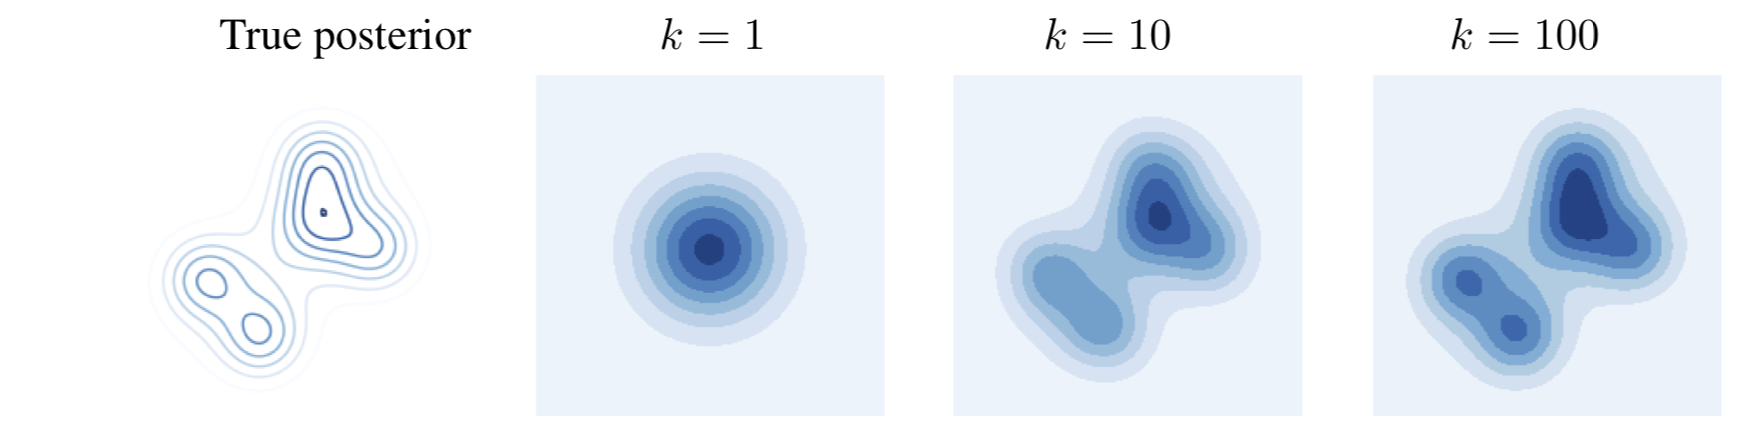
\includegraphics[width=\linewidth]{figs/IWAE_1.png}
		\end{figure}
	\end{block}

	\myfootnotewithlink{https://arxiv.org/abs/1704.02916}{Cremer C., Morris Q., Duvenaud D. Reinterpreting Importance-Weighted Autoencoders, 2017}
\end{frame}
%=======
\begin{frame}{IWAE}
	\begin{block}{Objective}
		\vspace{-0.5cm}
		\[
		\mathcal{L}_K (q, \btheta)  = \mathbb{E}_{\bz_1, \dots, \bz_K \sim q(\bz | \bx, \bphi)} \log \left( \frac{1}{K}\sum_{k=1}^K\frac{p(\bx, \bz_k | \btheta)}{q(\bz_k| \bx, \bphi)} \right) \rightarrow \max_{\bphi, \btheta}.
		\]
		\vspace{-0.3cm}
	\end{block}
	\begin{block}{Gradient}
		\vspace{-0.3cm}
		\[
		\Delta_K = \nabla_{\btheta, \bphi} \log \left( \frac{1}{K}\sum_{k=1}^K\frac{p(\bx, \bz_k | \btheta)}{q(\bz_k| \bx, \bphi)} \right), \quad \bz_k \sim q(\bz | \bx, \bphi).
		\]
		\vspace{-0.3cm}
	\end{block}
	\begin{block}{Theorem}
		\vspace{-0.4cm}
		\[
			\text{SNR}_K = \frac{\bbE [\Delta_K]}{\sigma(\Delta_K)}; \quad
			\text{SNR}_K(\btheta) = O(\sqrt{K}); \quad 
			\text{SNR}_K(\bphi) = O\left(\sqrt{\frac{1}{K}}\right).
		\]
		Hence, increasing $K$ vanishes gradient signal of inference network $q(\bz | \bx, \bphi)$.
	\end{block}

	\myfootnotewithlink{https://arxiv.org/abs/1802.04537}{Rainforth T. et al. Tighter variational bounds are not necessarily better, 2018}
\end{frame}
%=======
\begin{frame}{IWAE}
	\begin{block}{Theorem}
		\vspace{-0.5cm}
		\[
			\text{SNR}_K = \frac{\bbE [\Delta_K]}{\sigma(\Delta_K)}; \quad
			\text{SNR}_K(\btheta) = O(\sqrt{K}); \quad 
			\text{SNR}_K(\bphi) = O\left(\sqrt{\frac{1}{K}}\right).
		\]
		\vspace{-0.8cm}
	\end{block}
		\begin{minipage}[t]{0.5\columnwidth}
			\begin{figure}[h]
				\centering
				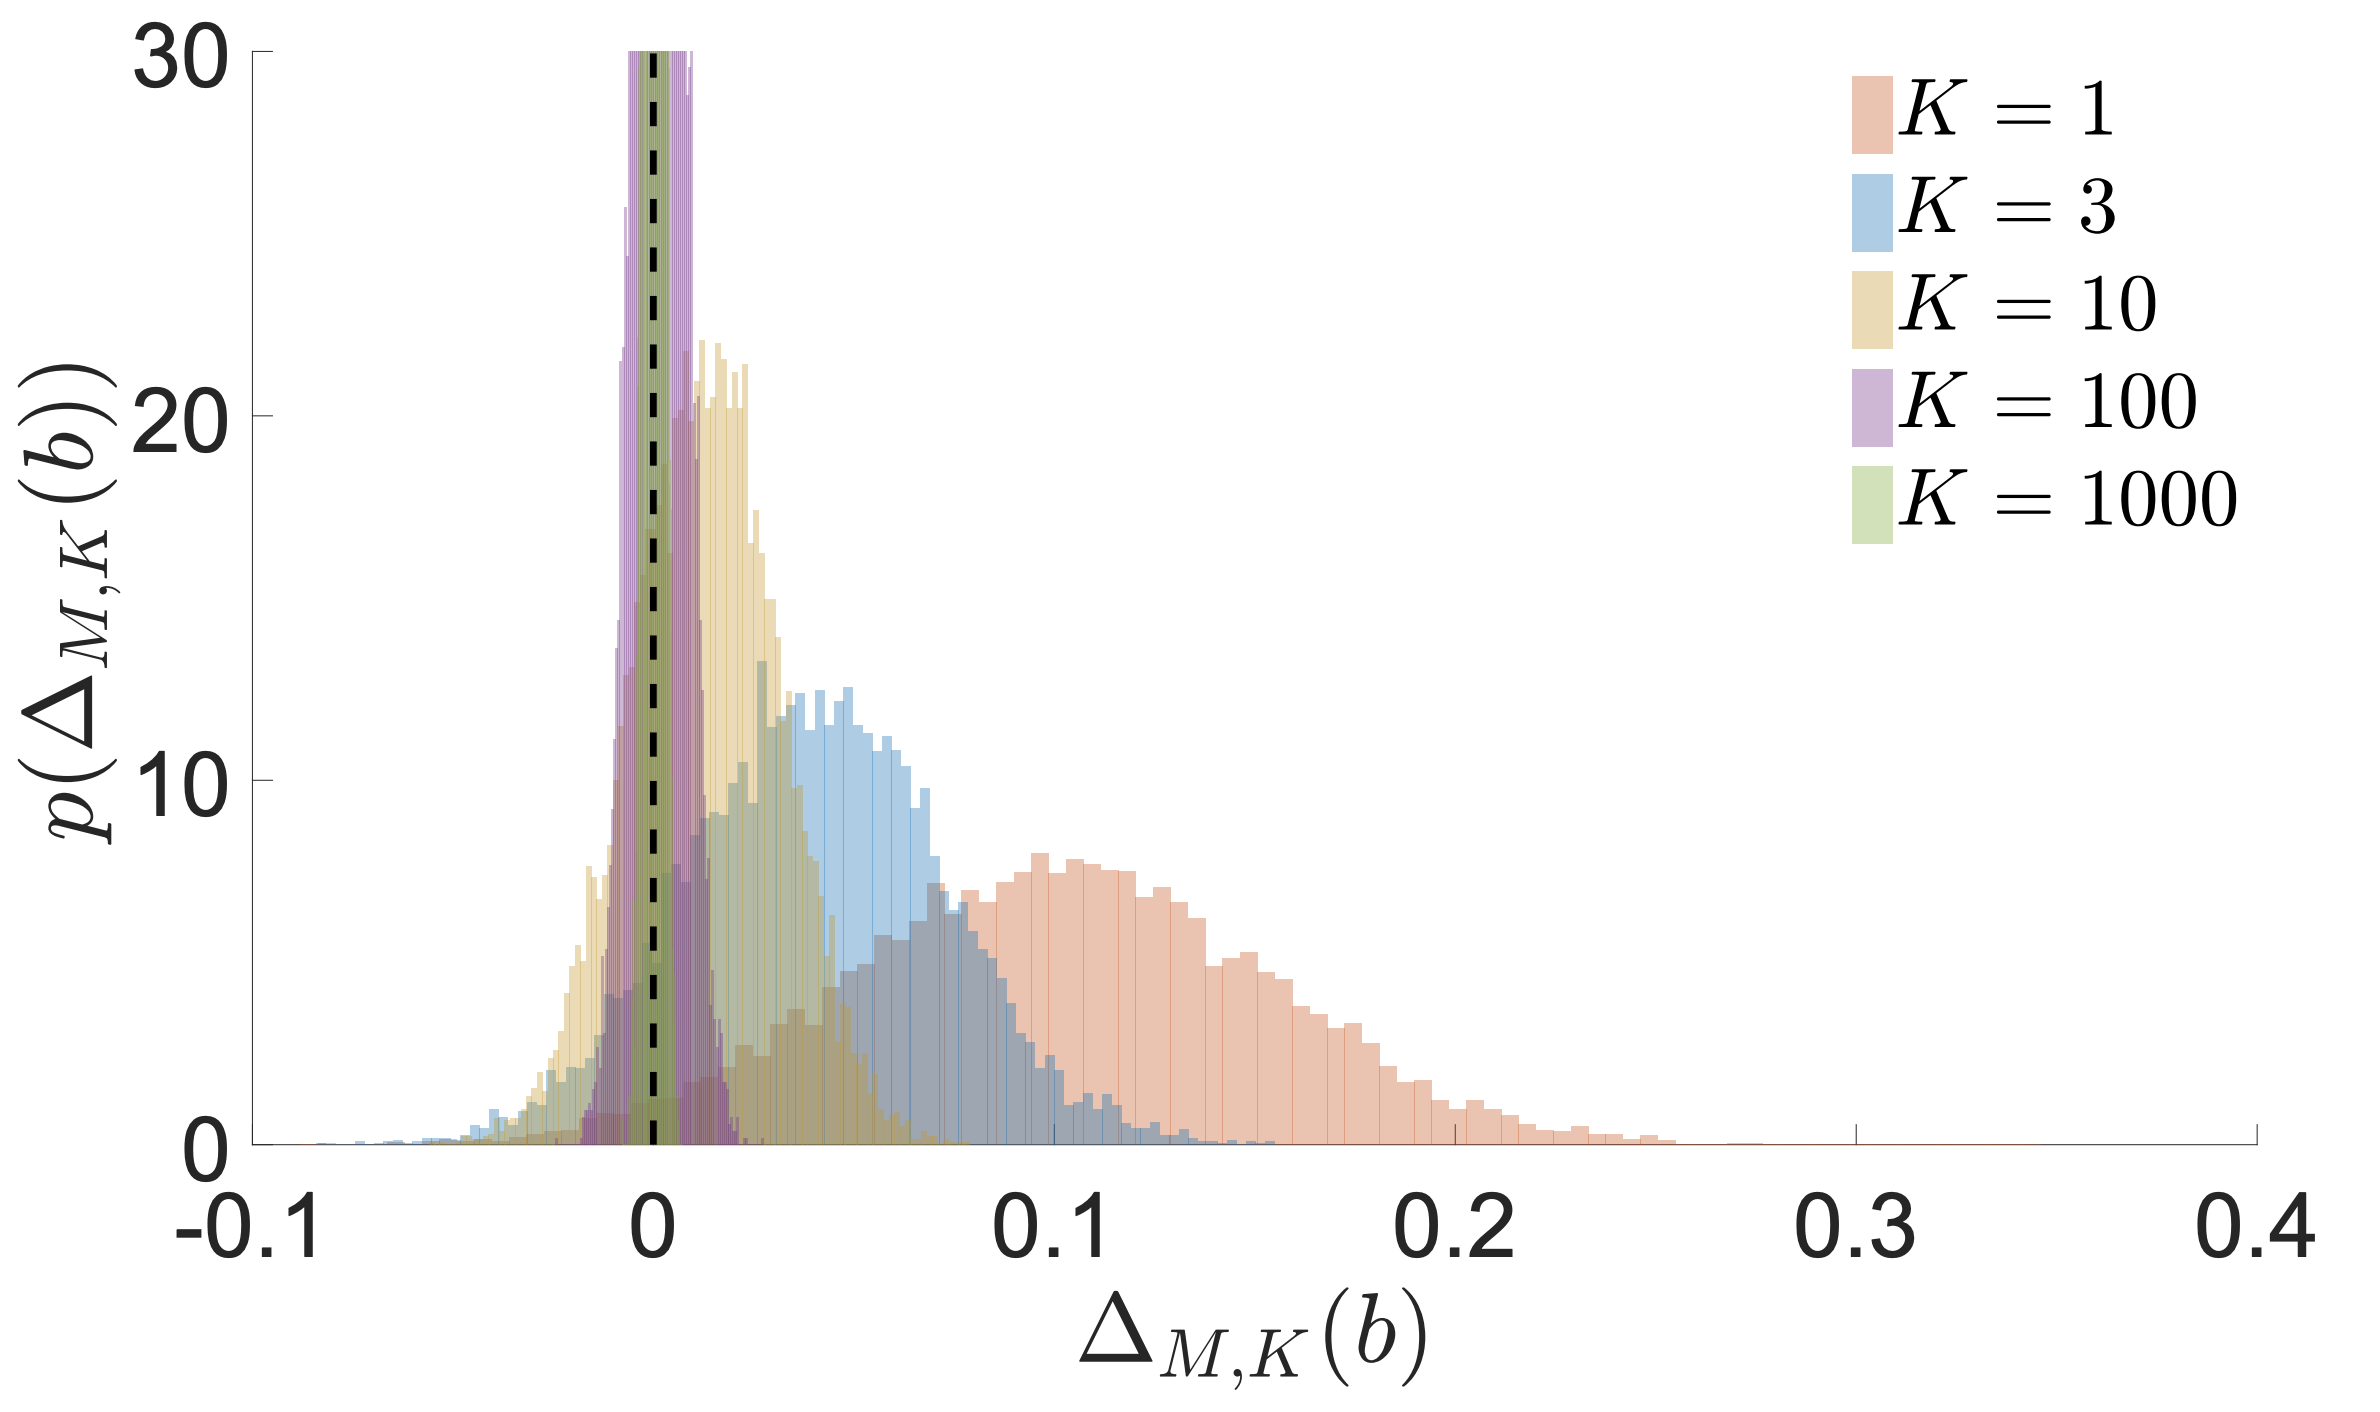
\includegraphics[width=1.\linewidth]{figs/IWAE_SNR_1.png}
			\end{figure}
		\end{minipage}%
		\begin{minipage}[t]{0.5\columnwidth}
			\begin{figure}[h]
				\centering
				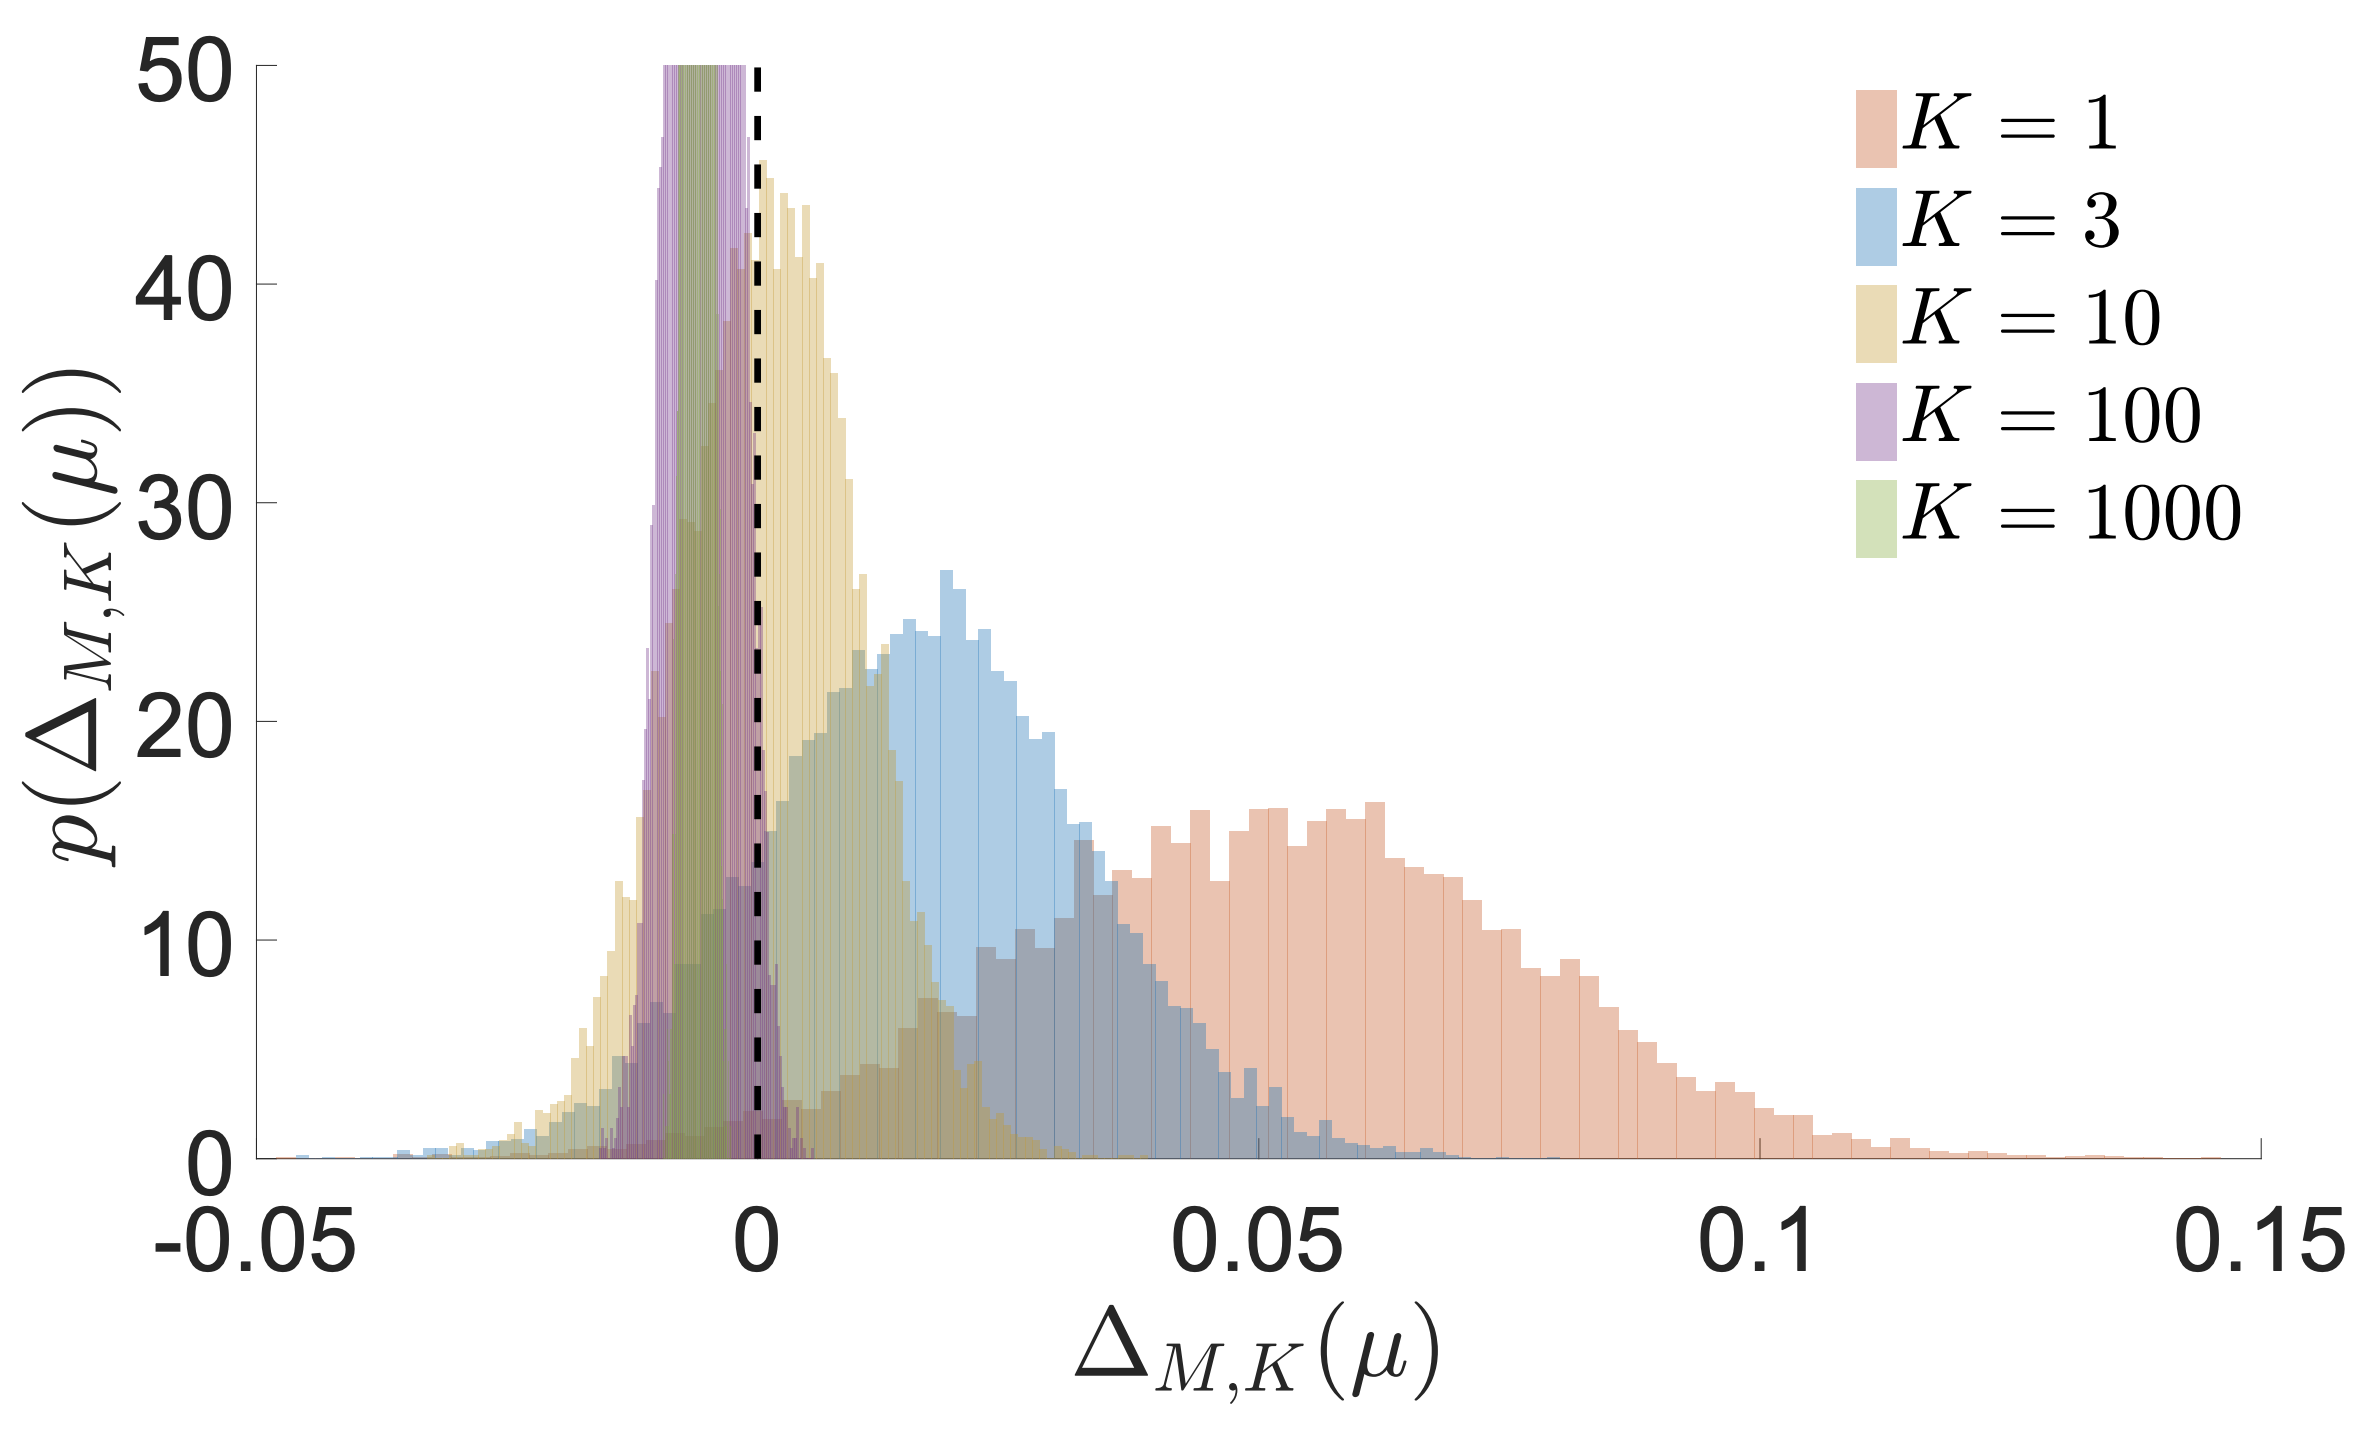
\includegraphics[width=1.\linewidth]{figs/IWAE_SNR_2.png}
			\end{figure}
		\end{minipage}
	\begin{itemize}
		\item IWAE makes the variational bound tighter and extends the class of variational distributions.
		\item Gradient signal becomes really small, training is complicated.
		\item IWAE is very popular technique as a quality measure for VAE models.
	\end{itemize}
	\myfootnotewithlink{https://arxiv.org/abs/1802.04537}{Rainforth T. et al. Tighter variational bounds are not necessarily better, 2018}
\end{frame}
%=======
\begin{frame}{VAE limitations}
	\begin{itemize}
		\item Poor variational posterior distribution (encoder)
		\[
			q(\bz | \bx, \bphi) = \mathcal{N}(\bz| \bmu_{\bphi}(\bx), \bsigma^2_{\bphi}(\bx)).
		\]
		\item Poor prior distribution
		\[
			p(\bz) = \mathcal{N}(0, \mathbf{I}).
		\]
		\item Poor probabilistic model (decoder)
		\[
			p(\bx | \bz, \btheta) = \mathcal{N}(\bx| \bmu_{\btheta}(\bz), \bsigma^2_{\btheta}(\bz)).
		\]
		\item Loose lower bound
		\[
			\log p(\bx | \btheta) - \mathcal{L}(q, \btheta) = (?).
		\]
	\end{itemize}
\end{frame}
%=======
\begin{frame}{ELBO interpretations}
	\[
		\log p(\bx | \btheta) = \cL (\bphi, \btheta) + KL(q(\bz | \bx, \bphi) || p(\bz | \bx, \btheta)) \geq  \cL (\bphi, \btheta).
	\]
	\[
		\cL (\bphi, \btheta) = \int q(\bz | \bx, \bphi) \log \frac{p(\bx, \bz | \btheta)}{q(\bz | \bx, \bphi)} d \bz.
	\]
	\begin{itemize}
	    \item Evidence minus posterior KL
	    \[
	        \mathcal{L}(q, \btheta) = \log p(\bx | \btheta) - KL(q(\bz | \bx, \bphi) || p(\bz | \bx, \btheta)).
	    \]
	    \item Average reconstruction loss with regularizer (prior KL)
	    \begin{align*}
	        \mathcal{L}(q, \btheta) &= \mathbb{E}_{q(\bz | \bx, \bphi)} \left[ \log p(\bx | \bz, \btheta) + \log p(\bz) - \log q(\bz | \bx, \bphi) \right] \\
	        &= \mathbb{E}_{q(\bz | \bx, \bphi)} \log p(\bx | \bz, \btheta) - KL(q(\bz | \bx, \bphi) || p(\bz)).
	    \end{align*}
	\end{itemize}
\end{frame}
%=======
\begin{frame}{ELBO surgery}
	\vspace{-0.3cm}
	\[
	    \frac{1}{n} \sum_{i=1}^n \mathcal{L}_i(q, \btheta) = \frac{1}{n} \sum_{i=1}^n \left[ \mathbb{E}_{q(\bz | \bx_i)} \log p(\bx_i | \bz, \btheta) - KL(q(\bz | \bx_i) || p(\bz)) \right].
	\]
	\vspace{-0.3cm}
	\begin{block}{Theorem}
		\[
		    \frac{1}{n} \sum_{i=1}^n KL(q(\bz | \bx_i) || p(\bz)) = KL(q(\bz) || p(\bz)) + \bbI_{q} [\bx, \bz],
		\]
		\begin{itemize}
			\item $q(\bz) = \frac{1}{n} \sum_{i=1}^n q(\bz | \bx_i)$ -- \textbf{aggregated} posterior distribution.
			\item $\bbI_{q} [\bx, \bz]$ -- mutual information between $\bx$ and $\bz$ under empirical data distribution and distribution $q(\bz | \bx)$.
			\item First term pushes $q(\bz)$ towards the prior $p(\bz)$.
			\item Second term reduces the amount of	information about $\bx$ stored in $\bz$. 
		\end{itemize}
	\end{block}
	\myfootnotewithlink{http://approximateinference.org/accepted/HoffmanJohnson2016.pdf}{Hoffman M. D., Johnson M. J. ELBO surgery: yet another way to carve up the variational evidence lower bound, 2016}
\end{frame}
%=======
\begin{frame}{ELBO surgery}
	\begin{block}{Theorem}
		\vspace{-0.3cm}
		\[
		    \frac{1}{n} \sum_{i=1}^n KL(q(\bz | \bx_i) || p(\bz)) = KL(q(\bz) || p(\bz)) + \bbI_q [\bx, \bz].
		\]
		\vspace{-0.4cm}
	\end{block}
	\begin{block}{Proof}
		\vspace{-0.5cm}
		{\footnotesize
		\begin{multline*}
		    \frac{1}{n} \sum_{i=1}^n KL(q(\bz | \bx_i) || p(\bz)) = \frac{1}{n} \sum_{i=1}^n \int q(\bz | \bx_i) \log \frac{q(\bz | \bx_i)}{p(\bz)} d \bz = \\
		    = \frac{1}{n} \sum_{i=1}^n \int q(\bz | \bx_i) \log \frac{q(\bz) q(\bz | \bx_i)}{p(\bz)q(\bz)} d \bz 
		    = \int \frac{1}{n} \sum_{i=1}^n  q(\bz | \bx_i) \log \frac{q(\bz)}{p(\bz)} d \bz + \\ 
		    + \frac{1}{n}\sum_{i=1}^n \int q(\bz | \bx_i) \log \frac{q(\bz | \bx_i)}{q(\bz)} d \bz = 
		     KL (q(\bz) || p(\bz)) + \frac{1}{n}\sum_{i=1}^n KL(q(\bz | \bx_i) || q (\bz))
		\end{multline*}
		}
		Without proof:
		\vspace{-0.4cm}
		\[
			\bbI_{q} [\bx, \bz] = \frac{1}{n}\sum_{i=1}^n KL(q(\bz | \bx_i) || q (\bz)) \in [0, \log n].
		\]
	\end{block}

	\myfootnotewithlink{http://approximateinference.org/accepted/HoffmanJohnson2016.pdf}{Hoffman M. D., Johnson M. J. ELBO surgery: yet another way to carve up the variational evidence lower bound, 2016}
\end{frame}
%=======
\begin{frame}{ELBO surgery}
	\begin{block}{ELBO revisiting}
		\vspace{-0.7cm}
		\begin{multline*}
		    \frac{1}{n}\sum_{i=1}^n \cL_i(q, \btheta) = \frac{1}{n} \sum_{i=1}^n \left[ \mathbb{E}_{q(\bz | \bx_i)} \log p(\bx_i | \bz, \btheta) - KL(q(\bz | \bx_i) || p(\bz)) \right] = \\
		    = \underbrace{\frac{1}{n} \sum_{i=1}^n \mathbb{E}_{q(\bz | \bx_i)} \log p(\bx_i | \bz, \btheta)}_{\text{Reconstruction loss}} - \underbrace{\vphantom{ \sum_{i=1}^n} \bbI_q [\bx, \bz]}_{\text{MI}} - \underbrace{\vphantom{ \sum_{i=1}^n} KL(q(\bz) || p(\bz))}_{\text{Marginal KL}}
		\end{multline*}
		\vspace{-0.3cm}
	\end{block}
	Prior distribution $p(\bz)$ is only in the last term.
	\begin{block}{Optimal VAE prior}
		\vspace{-0.3cm}
		\[
	  		KL(q(\bz) || p(\bz)) = 0 \quad \Leftrightarrow \quad p (\bz) = q(\bz) = \frac{1}{n} \sum_{i=1}^n q(\bz | \bx_i).
		\]
		The optimal prior $p(\bz)$ is the aggregated posterior $q(\bz)$.
	\end{block}
	
	\myfootnotewithlink{http://approximateinference.org/accepted/HoffmanJohnson2016.pdf}{Hoffman M. D., Johnson M. J. ELBO surgery: yet another way to carve up the variational evidence lower bound, 2016}
\end{frame}
%=======
\begin{frame}{Optimal VAE prior}
	How to choose the optimal $p(\bz)$?
	\begin{itemize}
		\item Standard Gaussian $p(\bz) = \mathcal{N}(0, I)$ $\Rightarrow$ over-regularization;
		\item $p(\bz) = q(\bz) = \frac{1}{n}\sum_{i=1}^n q(\bz | \bx_i)$ $\Rightarrow$ overfitting and highly expensive.
	\end{itemize}
	\vspace{-0.3cm}
	\begin{minipage}[t]{0.5\columnwidth}
		\begin{block}{Non learnable prior $p(\bz)$}
			\begin{figure}[h]
				\centering
				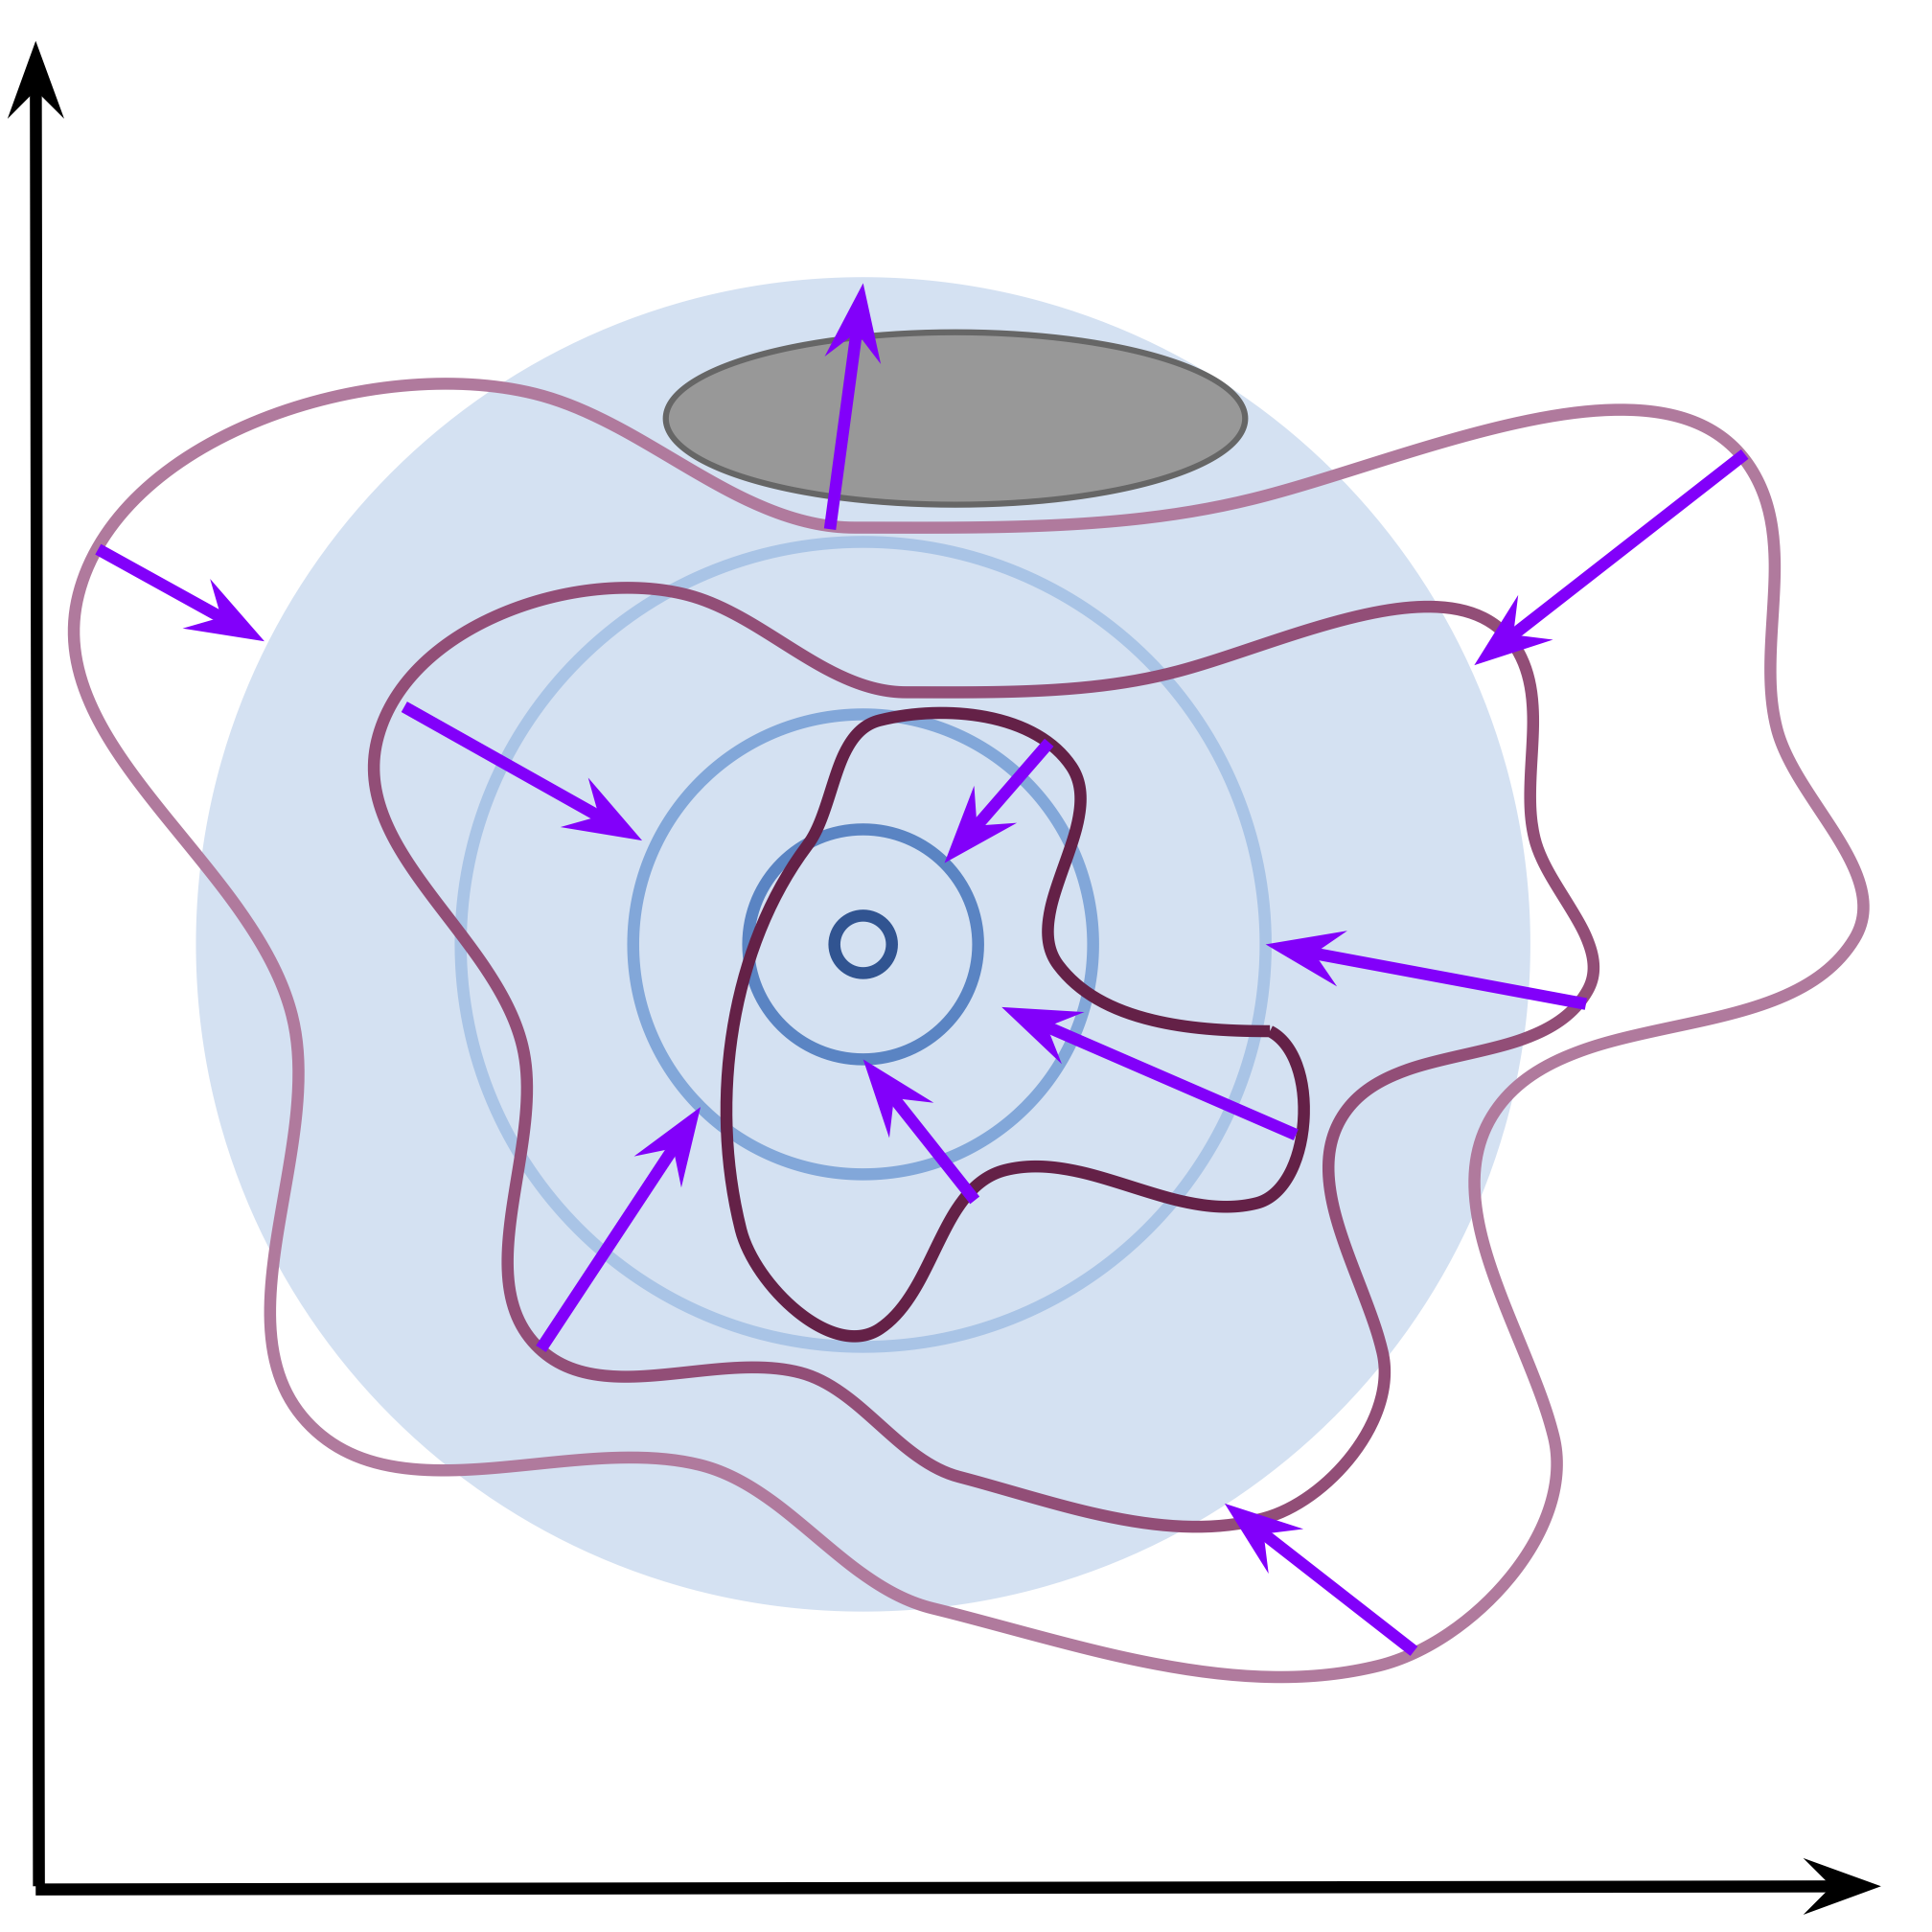
\includegraphics[width=0.8\linewidth]{figs/non_learnable_prior}
			\end{figure}
		\end{block}
	\end{minipage}%
	\begin{minipage}[t]{0.5\columnwidth}
		\begin{block}{Learnable prior $p(\bz | \blambda)$}
			\begin{figure}[h]
				\centering
				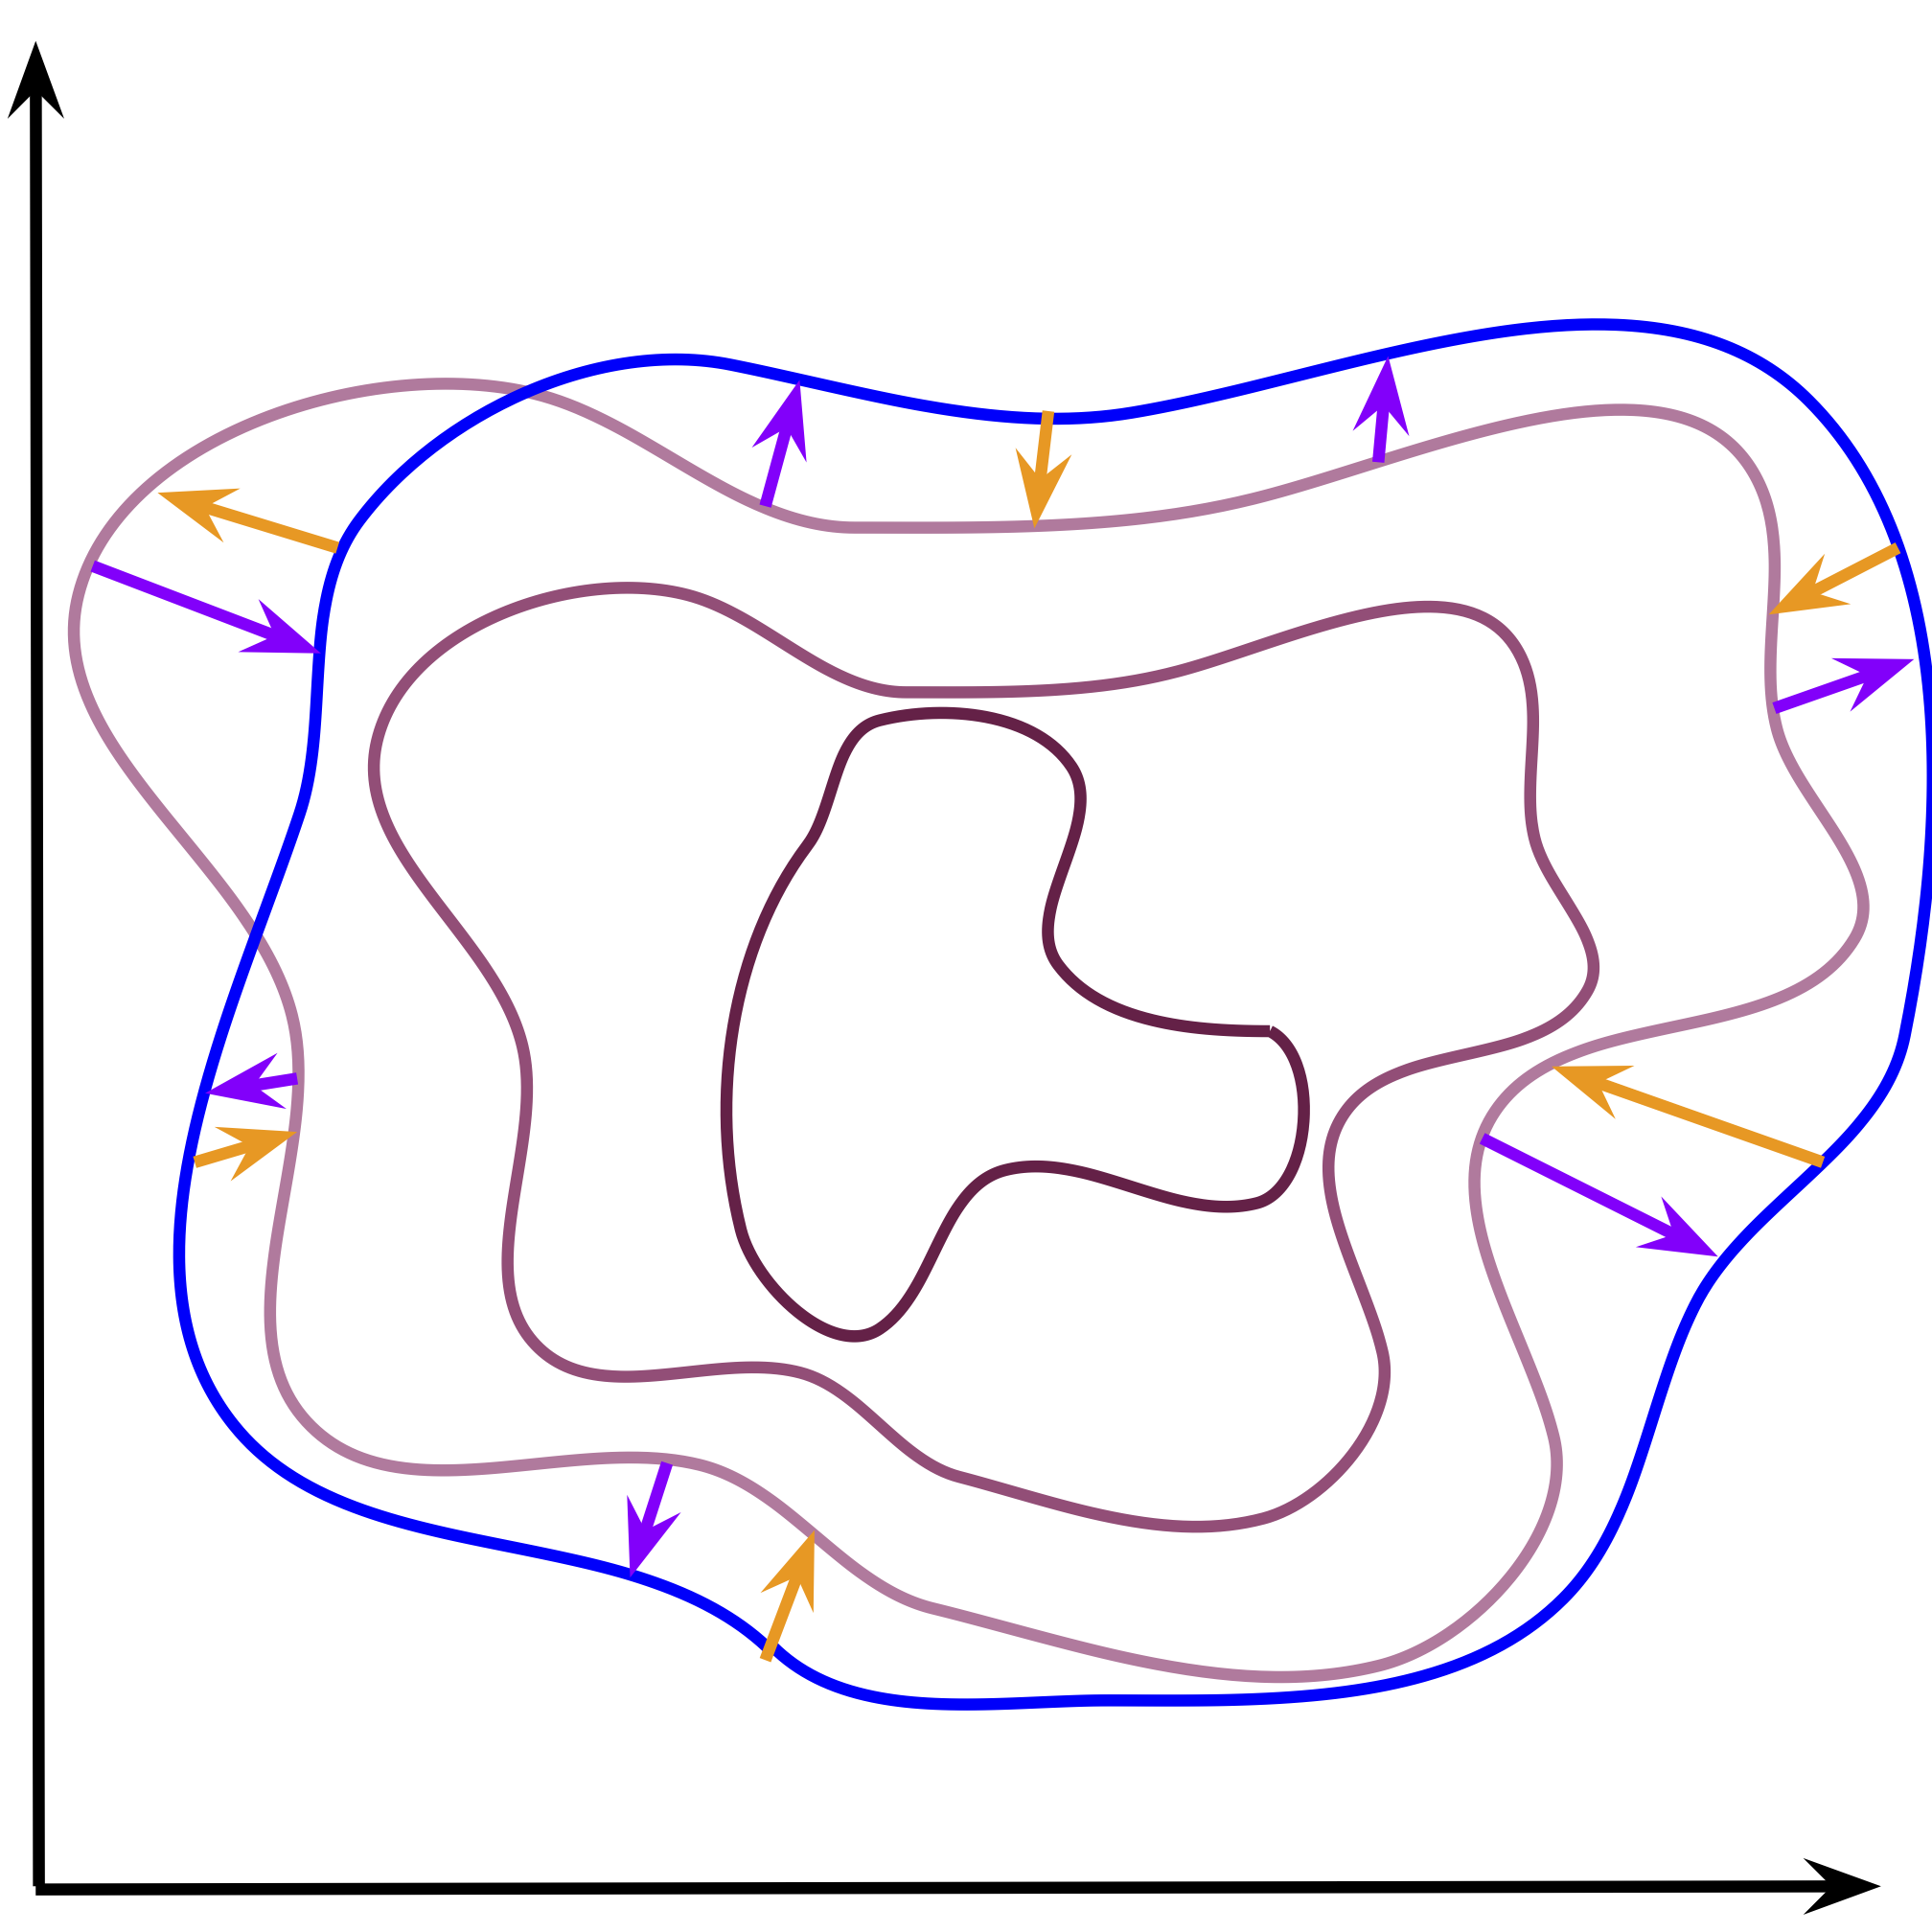
\includegraphics[width=0.8\linewidth]{figs/learnable_prior}
			\end{figure}
		\end{block}
	\end{minipage}
	\myfootnotewithlink{https://jmtomczak.github.io/blog/7/7\_priors.html}{image credit: https://jmtomczak.github.io/blog/7/7\_priors.html}
\end{frame}
%=======
\begin{frame}{Learnable VAE prior}
	\begin{block}{Optimal prior}
		\vspace{-0.4cm}
		\[
			KL(q(\bz) || p(\bz)) = 0 \quad \Leftrightarrow \quad p (\bz) = q(\bz) = \frac{1}{n} \sum_{i=1}^n q(\bz | \bx_i).
		\]
		\vspace{-0.4cm}
	\end{block}
	\begin{block}{Mixture of Gaussians}
		\vspace{-0.3cm}
		\[
			p(\bz | \blambda) = \sum_{k=1}^K w_k \cN(\bz | \bmu_k, \bsigma_k^2), \quad \blambda = \{\bw_k, \bmu_k, \bsigma_k\}_{k=1}^K.
		\]
		\vspace{-0.5cm}
	\end{block}
	\begin{block}{Variational Mixture of posteriors (VampPrior)}
		\vspace{-0.3cm}
		\[
		p(\bz | \blambda) = \frac{1}{K} \sum_{k=1}^K q(\bz | \bu_k),
		\]
		where $\blambda = \{\bu_1, \dots, \bu_K\}$ are trainable pseudo-inputs.
	\end{block}
	\begin{itemize}
		\item Multimodal $\Rightarrow$ prevents over-regularization;.
		\item $K \ll n$ $\Rightarrow$ prevents from potential overfitting + less expensive to train.
	\end{itemize}
	\myfootnotewithlink{https://arxiv.org/abs/1705.07120}{Tomczak J. M., Welling M. VAE with a VampPrior, 2017}
\end{frame}
%=======
\begin{frame}{VampPrior}
	\begin{itemize}
	\item Do we really need the multimodal prior?
	\item Is it beneficial to couple the prior with the variational posterior or the MoG prior is enough?
	\end{itemize}
	\begin{block}{Results}
		\vspace{-0.3cm}
		\begin{minipage}[t]{0.55\columnwidth}
			\begin{figure}[h]
				\centering
				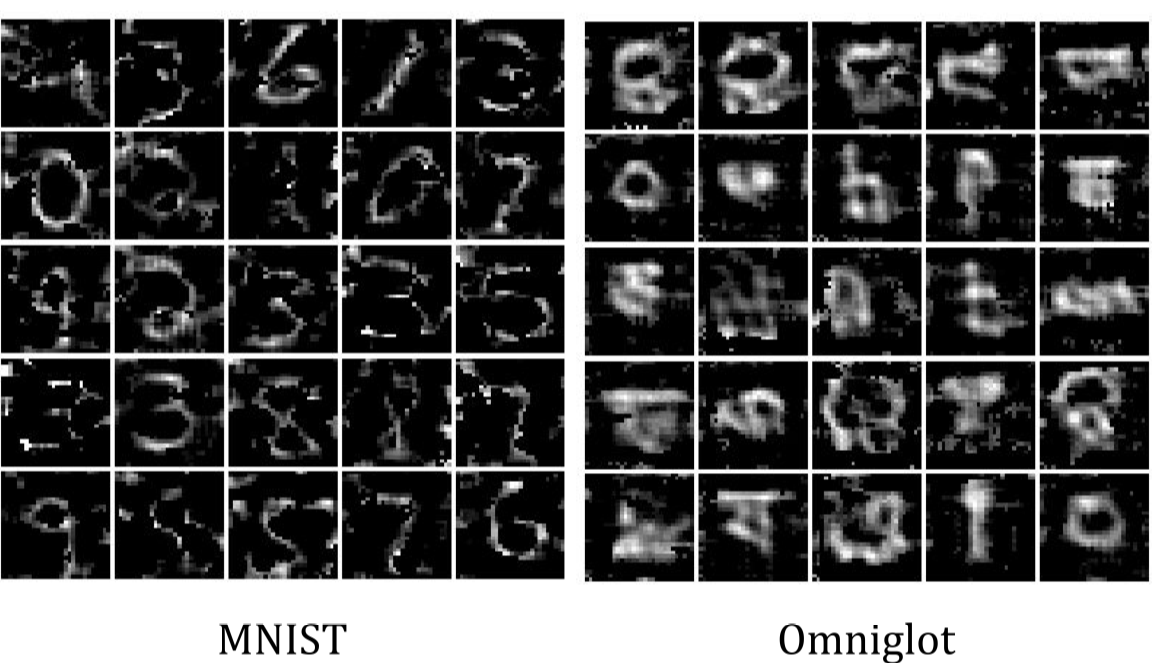
\includegraphics[width=1.0\linewidth]{figs/VampPrior_1.png}
			\end{figure}
		\end{minipage}%
		\begin{minipage}[t]{0.45\columnwidth}
			\begin{figure}[h]
				\centering
				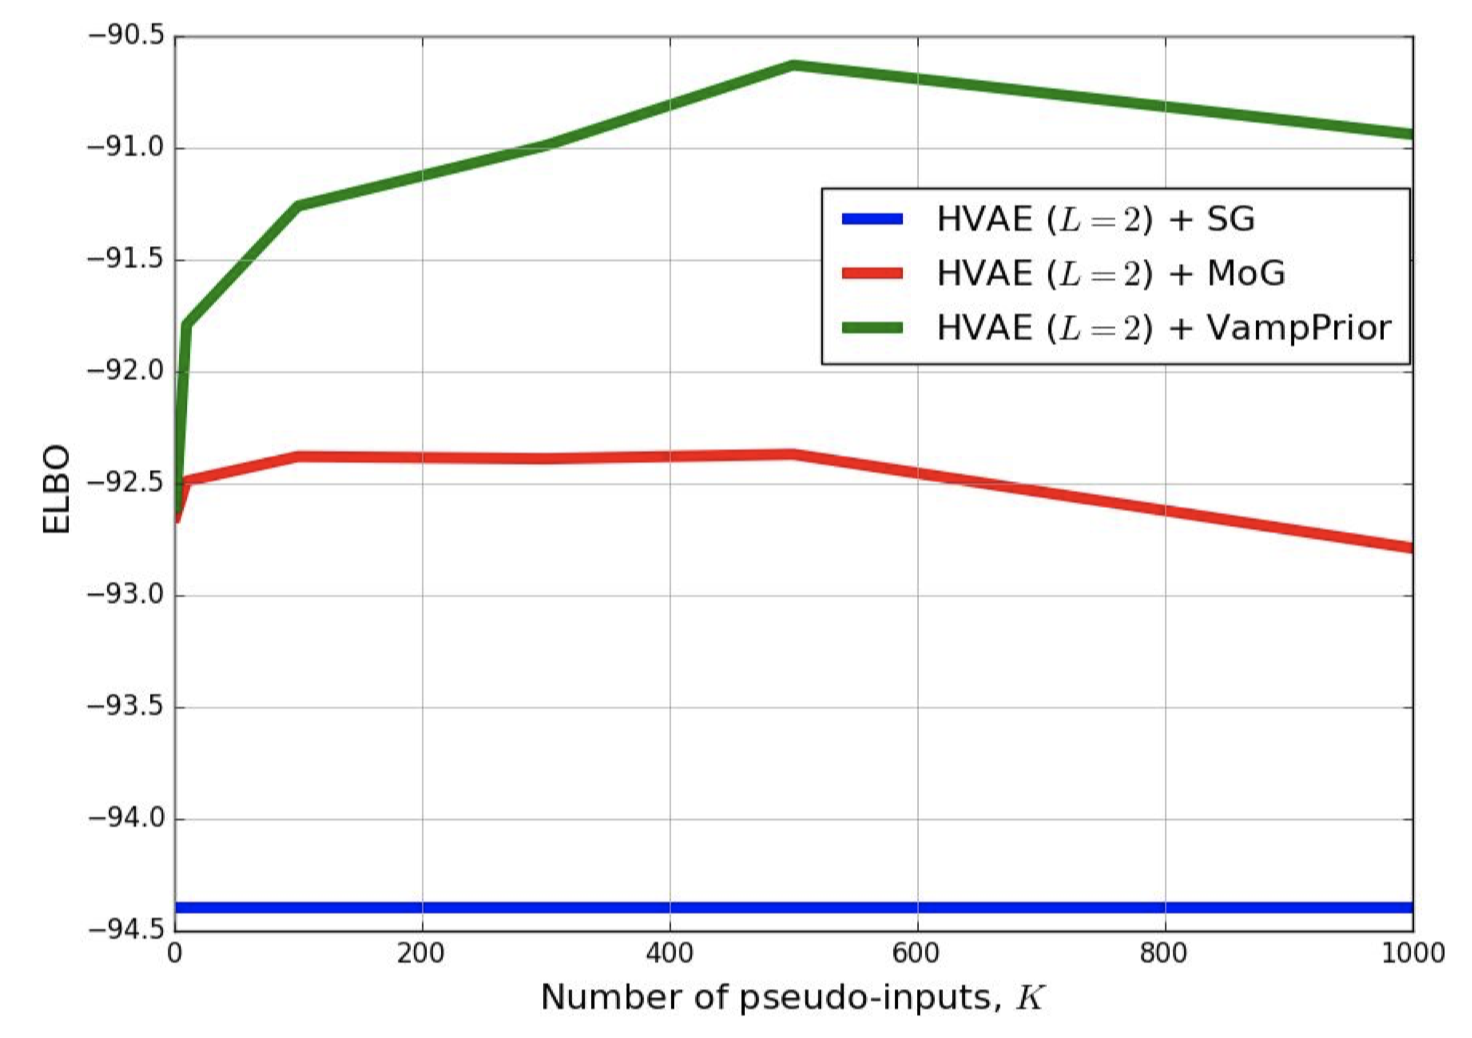
\includegraphics[width=1.0\linewidth]{figs/VampPrior_2.png}
			\end{figure}
		\end{minipage}
	\end{block}
	\textbf{Top row:} generated images by PixelHVAE + VampPrior for chosen pseudo-input in the left top corner. \\
	\vspace{0.1cm}
	\textbf{Bottom row:} pseudo-inputs for different datasets.
	\myfootnotewithlink{https://arxiv.org/abs/1705.07120}{Tomczak J. M., Welling M. VAE with a VampPrior, 2017}
\end{frame}
%=======
\begin{frame}{Flows-based VAE prior}
	\begin{block}{Flow model in latent space}
		\vspace{-0.3cm}
		\[
			\log p(\bz | \blambda) = \log p(\bepsilon) + \log \det \left | \frac{d \bepsilon}{d\bz}\right| = \log p(\bepsilon) + \log \det \left | \frac{\partial f(\bz, \blambda)}{\partial \bz}\right| 
		\]
		\[
			\bz = g(\bepsilon, \blambda) = f^{-1}(\bepsilon, \blambda)
		\]
	\end{block}
	\vspace{-0.3cm}
	\begin{itemize}
		\item RealNVP flow.
		\item Autoregressive flow (MAF).
	\end{itemize}
	Why it is not a good idea to use IAF for VAE prior?
	\begin{block}{ELBO with flow-based VAE prior}
		\vspace{-0.3cm}
		{\small
		\begin{multline*}
			\mathcal{L}(q, \btheta) = \mathbb{E}_{q(\bz | \bx)} \left[ \log p(\bx | \bz, \btheta) +  \log p(\bz | \blambda) - \log q(\bz | \bx) \right] \\
				= \mathbb{E}_{q(\bz | \bx)} \left[ \log p(\bx | \bz, \btheta) + \underbrace{ \Bigl( \log p(f(\bz, \blambda)) + \log \left| \det \frac{\partial f(\bz, \blambda)}{\partial \bz} \right| \Bigr) }_{\text{AF prior}} - \log q(\bz | \bx) \right] 
		\end{multline*}
		}
	\end{block}
	\myfootnotewithlink{https://arxiv.org/abs/1611.02731}{Chen X. et al. Variational Lossy Autoencoder, 2016}
\end{frame}
%=======
\begin{frame}{VAE limitations}
	\begin{itemize}
		\item Poor variational posterior distribution (encoder)
		\[
			q(\bz | \bx, \bphi) = \mathcal{N}(\bz| \bmu_{\bphi}(\bx), \bsigma^2_{\bphi}(\bx)).
		\]
		\item Poor prior distribution
		\[
			p(\bz) = \mathcal{N}(0, \mathbf{I}).
		\]
		\item Poor probabilistic model (decoder)
		\[
			p(\bx | \bz, \btheta) = \mathcal{N}(\bx| \bmu_{\btheta}(\bz), \bsigma^2_{\btheta}(\bz)).
		\]
		\item Loose lower bound
		\[
			\log p(\bx | \btheta) - \mathcal{L}(q, \btheta) = (?).
		\]
	\end{itemize}
\end{frame}
%=======
\begin{frame}{Variational posterior}
	\begin{block}{ELBO}
		\[
		\log p(\bx | \btheta) = \mathcal{L}(q, \btheta) + KL(q(\bz | \bx, \bphi) || p(\bz | \bx, \btheta)).
		\]
	\end{block}
	\begin{itemize}
		\item In E-step of EM-algorithm we wish $KL(q(\bz | \bx, \bphi) || p(\bz | \bx, \btheta)) = 0$. \\
		(In this case the lower bound is tight $\log p(\bx | \btheta) = \mathcal{L}(q, \btheta)$). \\
		\item Normal variational distribution $q(\bz | \bx, \bphi) = \mathcal{N}(\bz| \bmu_{\bphi}(\bx), \bsigma^2_{\bphi}(\bx))$ is poor (e.g. has only one mode). \\
		\item Flows models convert a simple base distribution to a complex one using invertible transformation with simple Jacobian. How to use flows in VAE posterior?
	\end{itemize}
\end{frame}
%=======
\begin{frame}{Flows in VAE posterior}
	Apply a sequence of transformations to the random variable
	\[
	\bz_0 \sim q(\bz | \bx, \bphi) = \mathcal{N}(\bz| \bmu_{\bphi}(\bx), \bsigma^2_{\bphi}(\bx)).
	\]
	Let $q(\bz | \bx, \bphi)$ (VAE encoder) be a base distribution for a flow model.
	
	\begin{block}{Flow model in latent space}
		\vspace{-0.3cm}
		\[
			\log q(\bz^* | \bx, \bphi, \blambda) = \log q(\bz | \bx, \bphi) + \log \det \left | \frac{\partial g(\bz, \blambda)}{\partial \bz}\right|
		\]
		\[
			\bz^* = g(\bz, \blambda) = f^{-1}(\bz, \blambda)
		\]
	\end{block}
	Here $g(\bz, \blambda)$ is a flow model (e.g. stack of planar/coupling layers) parameterized by $\blambda$.
	
	
	Let use $q(\bz^* | \bx, \bphi, \blambda)$ as a variational distribution. Here $\bphi$~-- encoder parameters, $\blambda$~-- flow parameters.
	
	\myfootnotewithlink{https://arxiv.org/abs/1505.05770}{Rezende D. J., Mohamed S. Variational Inference with Normalizing Flows, 2015} 
\end{frame}
%=======
\begin{frame}{Flows-based VAE posterior}
	\begin{itemize}
		\item Encoder outputs base distribution $q(\bz | \bx, \bphi)$.
		\item Flow model $\bz^* = g(\bz, \blambda)$ transforms the base distribution $q(\bz | \bx, \bphi)$ to the distribution $q(\bz^* | \bx, \bphi, \blambda)$.
		\item Distribution $q(\bz^* | \bx, \bphi, \blambda)$ is used as a variational distribution for ELBO maximization.
	\end{itemize}
	
	\begin{block}{Flow model in latent space}
		\vspace{-0.3cm}
		\[
			\log q(\bz^* | \bx, \bphi, \blambda) = \log q(\bz | \bx, \bphi) + \log \det \left | \frac{\partial g(\bz, \blambda)}{\partial \bz}\right|
		\]
		\vspace{-0.3cm}
	\end{block}
	\begin{block}{ELBO with flow-based VAE posterior}
		\vspace{-0.5cm}
		\begin{align*}
			\mathcal{L} (\bphi, \btheta, \blambda)  
			&= \bbE_{q(\bz^* | \bx, \bphi, \blambda)} \bigl[\log p(\bx, \bz^* | \btheta) - \log q(\bz^*| \bx, \bphi, \blambda) \bigr] \\ 
			&=  \bbE_{q(\bz^* | \bx, \bphi, \blambda)} \log p(\bx | \bz^*, \btheta) - KL (q(\bz^* | \bx, \bphi, \blambda) || p(\bz^*)).
		\end{align*}
		\vspace{-0.3cm}
	\end{block}
	The second term in ELBO is reverse KL divergence. Planar flows was originally proposed for variational inference in VAE.
	
	\myfootnotewithlink{https://arxiv.org/abs/1505.05770}{Rezende D. J., Mohamed S. Variational Inference with Normalizing Flows, 2015} 
\end{frame}
%=======
\begin{frame}{Flows-based VAE posterior}
	
	\begin{block}{Flow model in latent space}
		\vspace{-0.3cm}
		\[
			\log q(\bz^* | \bx, \bphi, \blambda) = \log q(\bz | \bx, \bphi) + \log \det \left | \frac{\partial g(\bz, \blambda)}{\partial \bz}\right|
		\]
		\vspace{-0.3cm}
	\end{block}
	\begin{block}{ELBO objective}
		\vspace{-0.5cm}
		\begin{multline*}
			\mathcal{L} (\bphi, \btheta, \blambda)  
			= \mathbb{E}_{q(\bz^* | \bx, \bphi, \blambda)} \bigl[\log p(\bx, \bz^* | \btheta) - \log q(\bz^*| \bx, \bphi, \blambda) \bigr] = \\
			= \mathbb{E}_{q(\bz | \bx, \bphi)} \left. \bigl[\log p(\bx, \bz^* | \btheta) - \log q(\bz^*| \bx, \bphi, \blambda) \bigr]\right|_{\bz^* = g(\bz, \blambda)} = \\
			= \mathbb{E}_{q(\bz | \bx, \bphi)} \bigg[\log p(\bx, \bz^* | \btheta) -  \log q(\bz | \bx, \bphi ) + \log \left| \det \left( \frac{\partial g(\bz, \blambda)}{\partial \bz} \right) \right| \bigg].
		\end{multline*}
	\end{block}
	\begin{itemize}
		\item Obtain samples $\bz$ from the encoder $q(\bz | \bx, \bphi)$.
		\item Apply flow model $\bz^* = g(\bz, \blambda)$.
		\item Compute likelihood for $\bz^*$ using the decoder, base distribution for $\bz^*$ and the Jacobian.
	\end{itemize}
	\myfootnotewithlink{https://arxiv.org/abs/1505.05770}{Rezende D. J., Mohamed S. Variational Inference with Normalizing Flows, 2015} 
\end{frame}
%=======
\begin{frame}{Inverse autoregressive flow (IAF)}
	\vspace{-0.3cm}
	\begin{align*}
		\bx &= g(\bz, \btheta) \quad \Rightarrow \quad x_i = \tilde{\sigma}_i (\bz_{1:i-1}) \cdot z_i + \tilde{\mu}_i(\bz_{1:i-1}). \\
		\bz &= f(\bx, \btheta) \quad \Rightarrow \quad z_i = \left(x_i - \tilde{\mu}_i(\bz_{1:i-1}) \right) \cdot \frac{1}{\tilde{\sigma}_i (\bz_{1:i-1})}.
	\end{align*}
	\vspace{-0.5cm}
	\begin{block}{Reverse KL for flow model}
  		\vspace{-0.5cm}
		\[
			KL(p || \pi)  = \bbE_{p(\bz)} \left[  \log p(\bz) - \log \left|\det \left( \frac{\partial g(\bz, \btheta)}{\partial \bz} \right) \right| - \log \pi(g(\bz, \btheta)) \right]
		\]
		\vspace{-0.3cm}
	\end{block}
	\begin{itemize}
	\item We don’t need to think about computing the function $f(\bx, \btheta)$.
	\item Inverse autoregressive flow is a natural choice for using flows in VAE:
	\end{itemize}
	\vspace{-0.3cm}
	\begin{align*}
		\bz &= \bsigma(\bx) \odot \bepsilon + \bmu(\bx), \quad \bepsilon \sim \mathcal{N}(0, 1); \quad  \sim q(\bz | \bx, \bphi). \\
		\bz_k &= \tilde{\bsigma}_k(\bz_{k - 1}) \odot \bz_{k-1} + \tilde{\bmu}_k(\bz_{k - 1}), \quad k \geq 1; \quad  \sim q_k(\bz_k | \bx, \bphi, \{\blambda_j\}_{j=1}^k).
	\end{align*}
	\myfootnotewithlink{https://arxiv.org/abs/1606.04934}{Kingma D. P. et al. Improving Variational Inference with Inverse Autoregressive Flow, 2016} 
\end{frame}
%=======
\begin{frame}{Inverse autoregressive flow (IAF)}
	\begin{figure}
		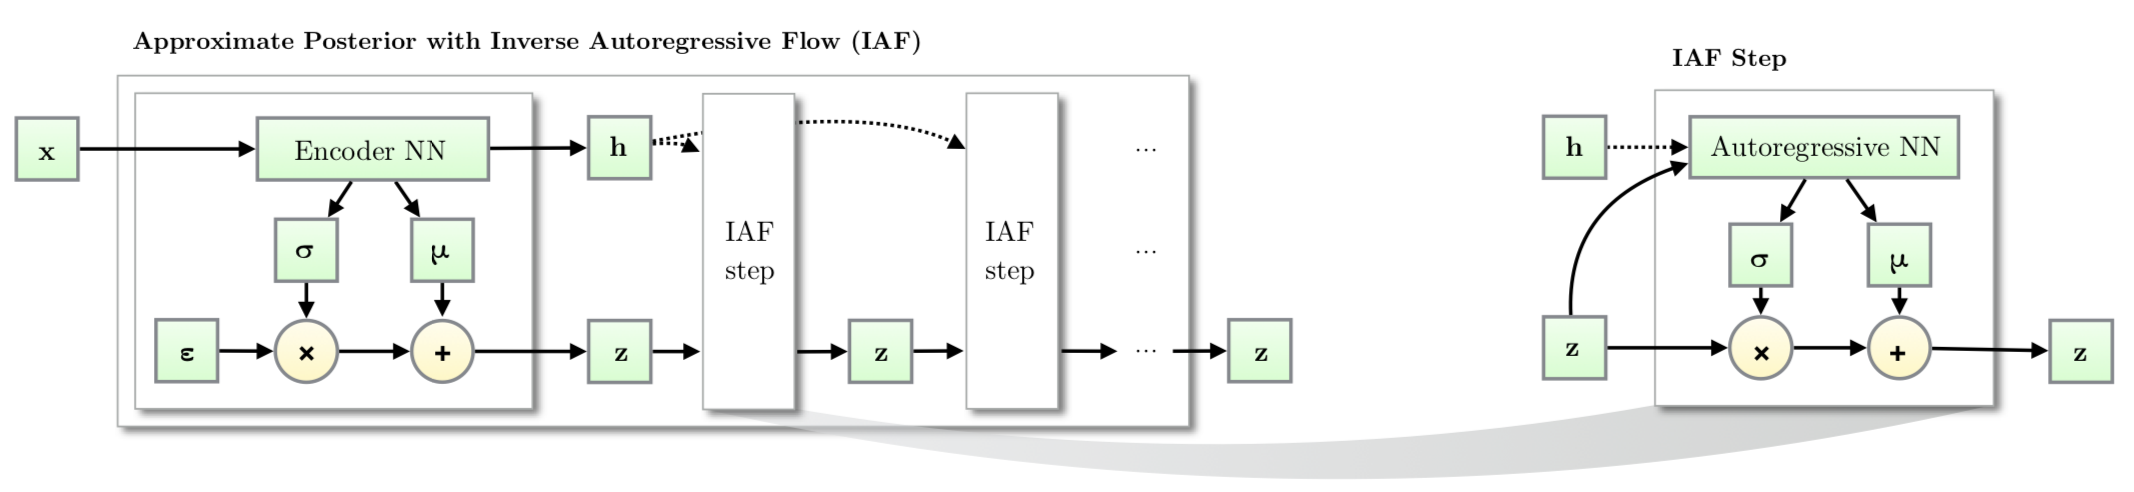
\includegraphics[width=\linewidth]{figs/iaf2.png}
	\end{figure}
	\begin{figure}
		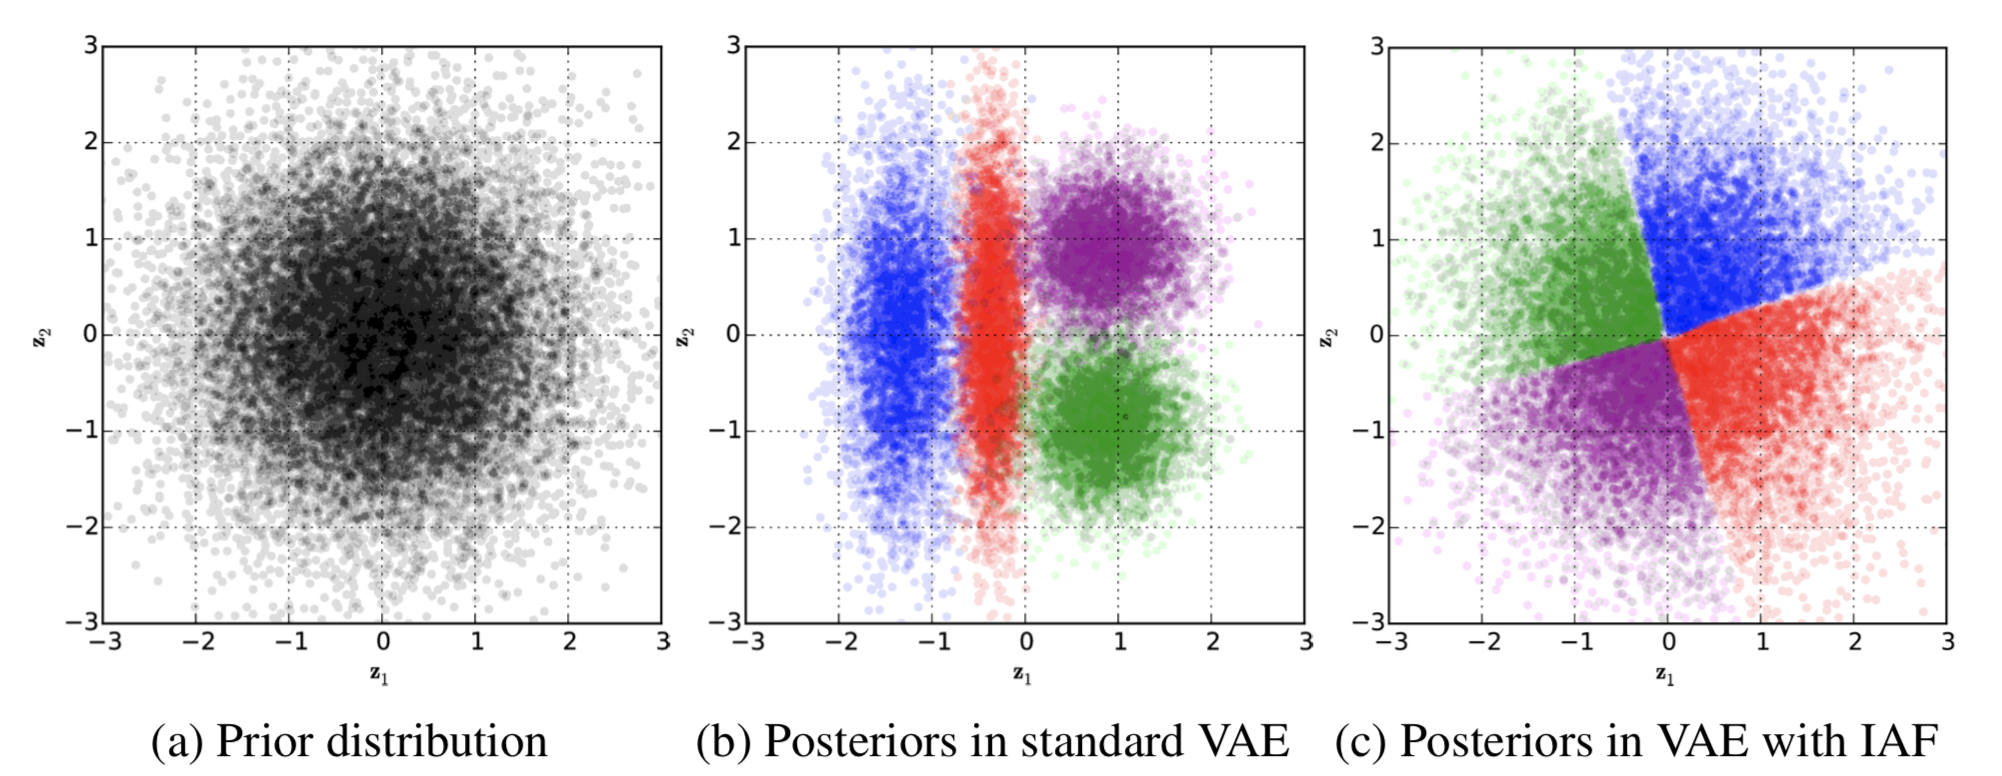
\includegraphics[width=\linewidth]{figs/iaf1.png}
	\end{figure}

	\myfootnotewithlink{https://arxiv.org/abs/1606.04934}{Kingma D. P. et al. Improving Variational Inference with Inverse Autoregressive Flow, 2016} 
\end{frame}
%=======
\begin{frame}{Flows-based VAE prior vs Flow-based VAE posterior}
	\begin{block}{Theorem}
	VAE with the AF prior for latent code $\bz$ is equivalent to using the IAF posterior for latent code $\bepsilon$.
	\end{block}
	\begin{block}{Proof}
	\vspace{-0.5cm}
	{\footnotesize
	\begin{align*}
	\mathcal{L}(q, \btheta) &= \mathbb{E}_{q(\bz | \bx)} \left[ \log p(\bx | \bz, \btheta) +  \log p(\bz | \blambda) - \log q(\bz | \bx) \right] \\
	&= \mathbb{E}_{q(\bz | \bx)} \Bigl[ \log p(\bx | \bz, \btheta) + \underbrace{ \Bigl( \log p(f(\bz, \blambda)) + \log \left| \det \frac{\partial f(\bz, \blambda)}{\partial \bz} \right| \Bigr) }_{\text{AF prior}} - \log q(\bz | \bx) \Bigr] \\
	&= \mathbb{E}_{q(\bz | \bx)} \Bigl[ \log p(\bx | \bz, \btheta) +  \log p(f(\bz, \blambda)) - \underbrace{ \Bigl( \log q(\bz | \bx) - \log \left| \det \frac{\partial f(\bz, \blambda)}{\partial \bz} \right| \Bigr) }_{\text{IAF posterior}} \Bigr]
	\end{align*}
	}
	\end{block}
	\vspace{-0.5cm}
	\begin{block}{Flows in VAE posterior}
		\vspace{-0.3cm}
		{\footnotesize
		\[
			\mathcal{L} (\bphi, \btheta) 
			= \mathbb{E}_{q(\bz_0 | \bx, \bphi)} \bigg[\log p(\bx, \bz_K | \btheta) -  \log q(\bz_0 | \bx, \bphi ) +   \log \left| \det \left( \frac{\partial g(\bz_0, \bphi_*)}{\partial \bz_0} \right) \right| \bigg].
		\]
		}
	\end{block}
	\myfootnotewithlink{https://arxiv.org/abs/1611.02731}{Chen X. et al. Variational Lossy Autoencoder, 2016}
\end{frame}
%=======
\begin{frame}{Flows-based VAE prior vs Flow-based VAE posterior}
	\begin{block}{Autoregressive flow prior}
		{\footnotesize
		\begin{align*}
			\mathcal{L}(q, \btheta) &= \mathbb{E}_{\bz \sim q(\bz | \bx)} \Bigl[ \log p(\bx | \bz, \btheta) + \underbrace{ \Bigl( \log p(f(\bz, \blambda)) + \log \left| \det \frac{\partial f(\bz, \blambda)}{\partial \bz} \right| \Bigr) }_{\text{AF prior}} - \log q(\bz | \bx) \Bigr] \\
			&= \mathbb{E}_{\bz \sim q(\bz | \bx)} \Bigl[ \log p(\bx | \bz, \btheta) +  \log p(f(\bz, \blambda)) - \underbrace{ \Bigl( \log q(\bz | \bx) - \log \left| \det \frac{\partial f(\bz, \blambda)}{\partial \bz} \right| \Bigr) }_{\text{IAF posterior}} \Bigr]
		\end{align*}
		}
	\end{block}
	\begin{itemize}
		\item IAF posterior decoder path: $p(\bx|\bz, \btheta)$, $\bz \sim p(\bz)$.
		\item AF prior decoder path: $p(\bx|\bz, \btheta)$, $\bz = g(\bepsilon, \blambda)$, $\bepsilon \sim p(\bepsilon)$. 
	\end{itemize}
	The AF prior and the IAF posterior have the same computation cost, so using the AF prior makes the model more expressive at no training time cost.

	\myfootnotewithlink{https://arxiv.org/abs/1611.02731}{Chen X. et al. Variational Lossy Autoencoder, 2016}
\end{frame}
%=======
\begin{frame}{Summary}
	\begin{itemize}
		\item The IWAE could get the tighter lower bound to the likelihood, but the training of such model becomes more difficult.
		\vfill
		\item The ELBO surgery reveals insights about a prior distribution in VAE. The optimal prior is the aggregated posterior.
		\vfill
		\item VampPrior proposes to use a variational mixture of posteriors as the prior to approximate the aggregated posterior.
		\vfill
		\item The autoregressive flows could be used as the prior. This is equivalent to the use of the IAF posterior. 
	\end{itemize}
\end{frame}

\end{document} 